\chapter{Supplemental information for Chapter 1}

\begin{figure}
    \centering
    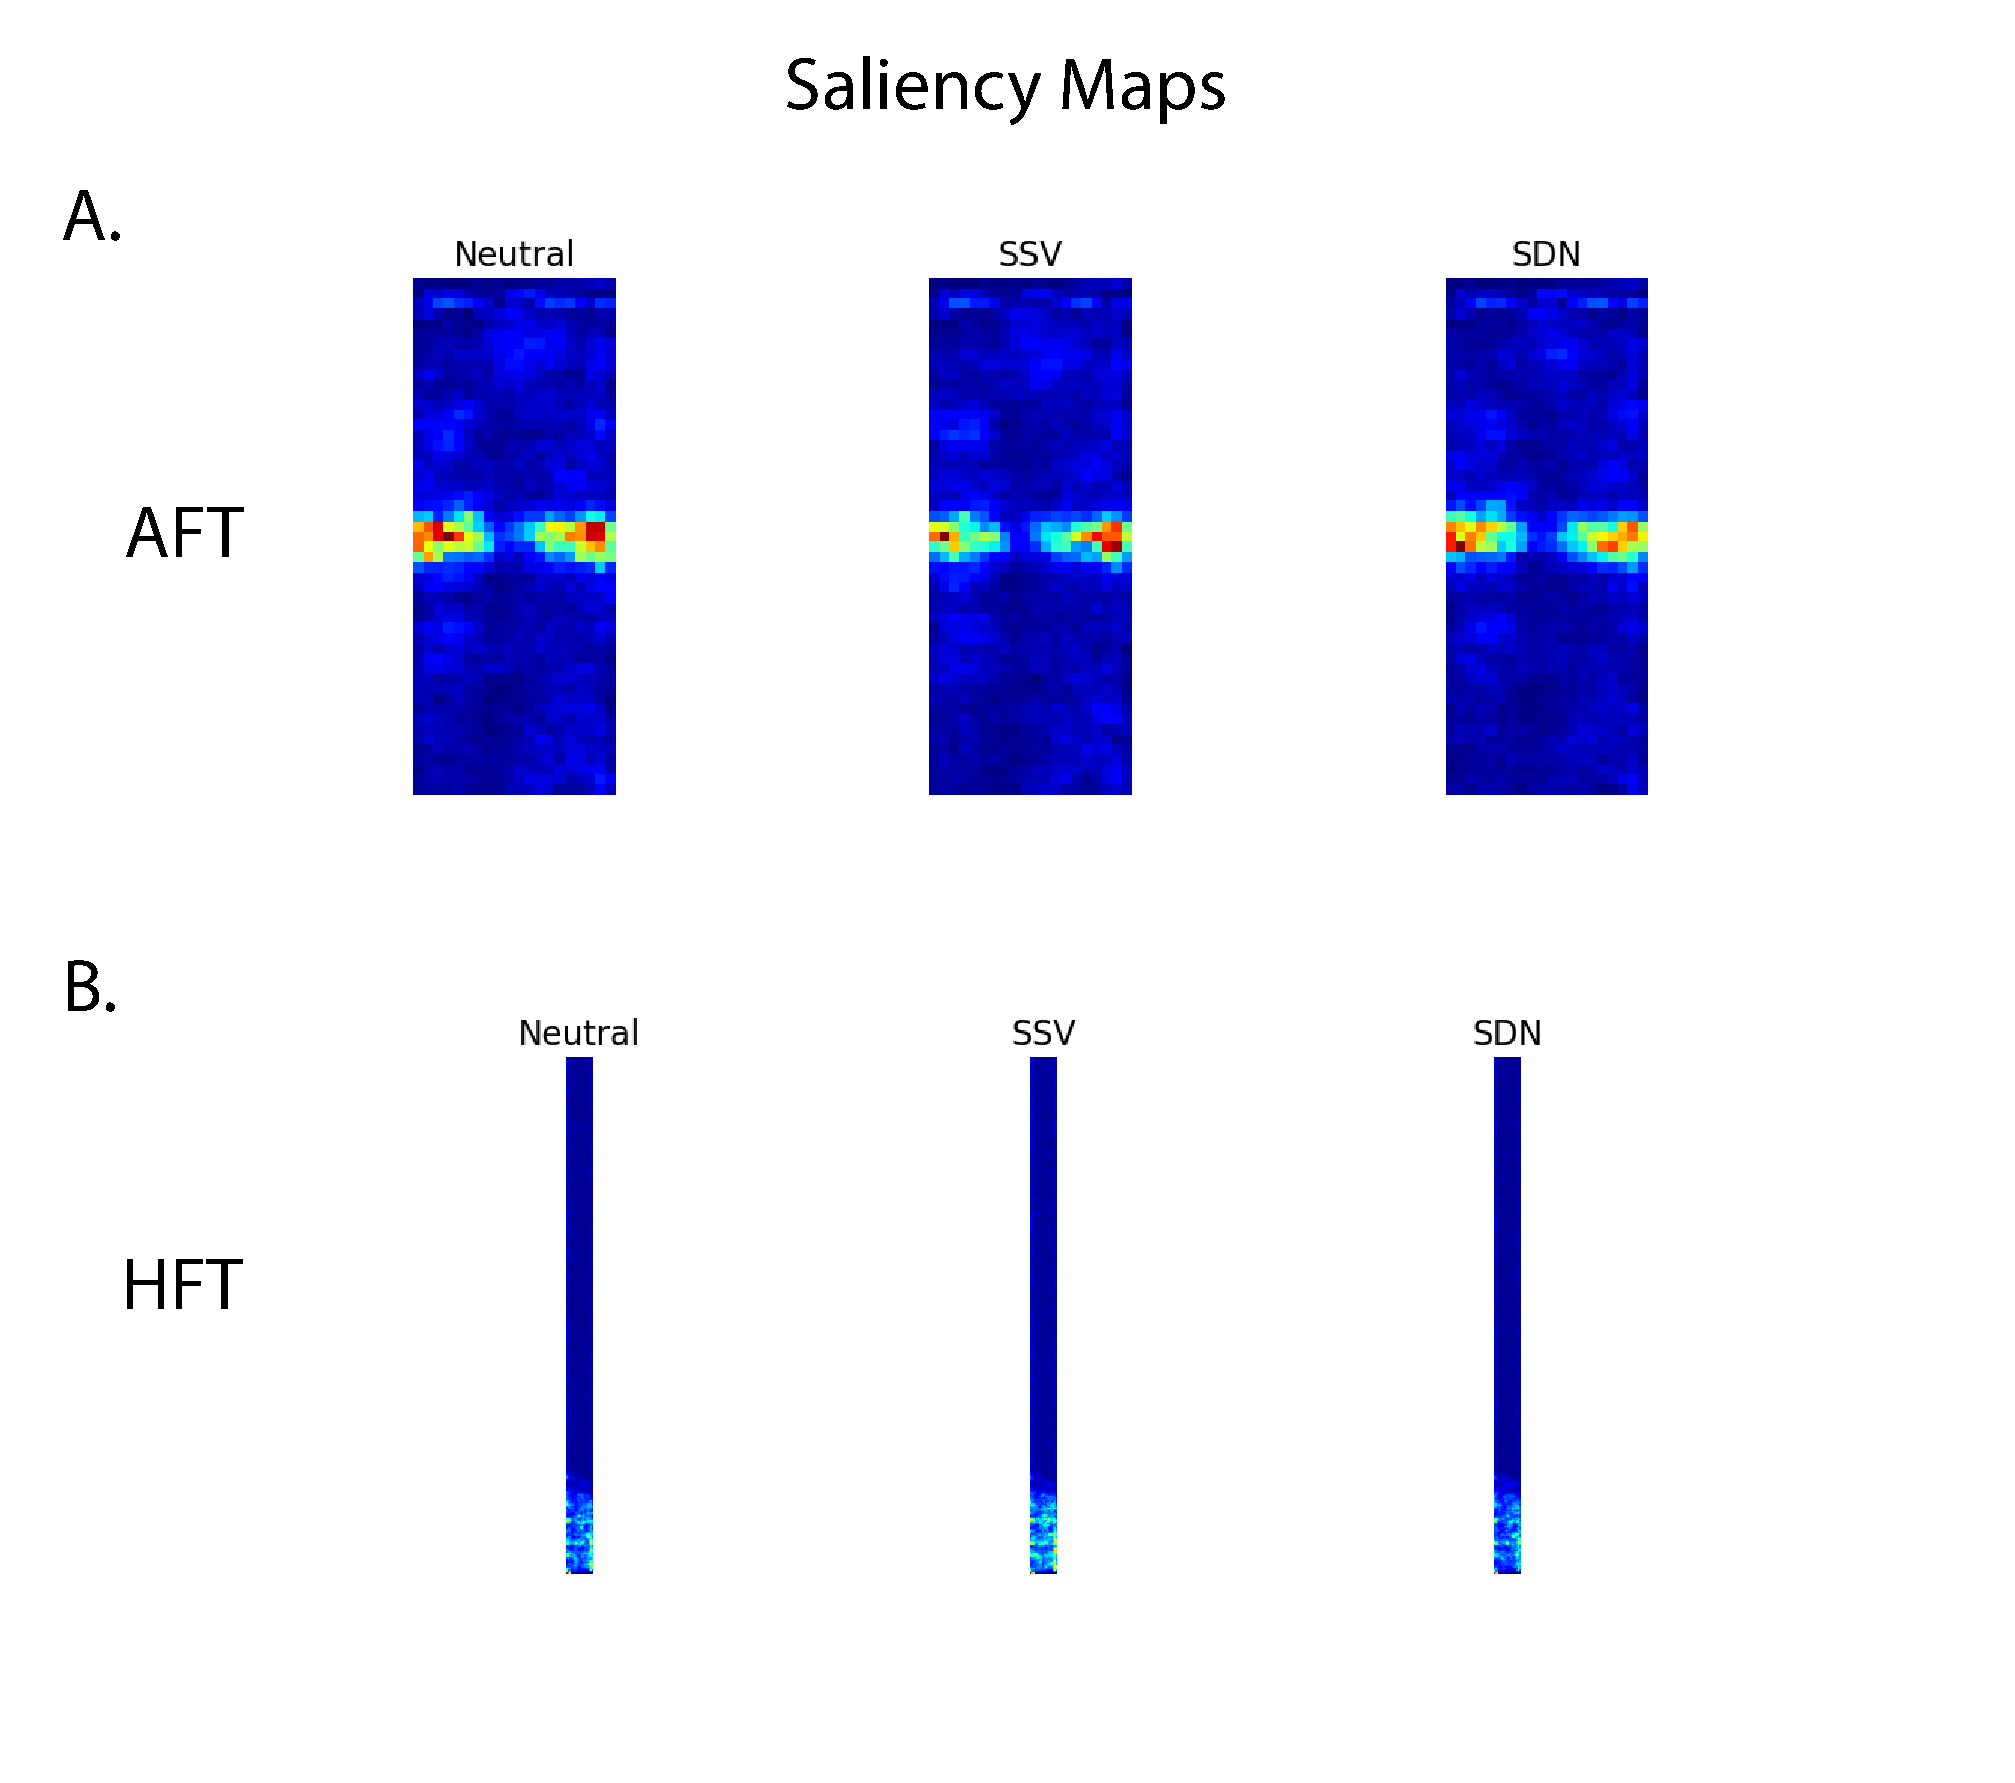
\includegraphics[width=\textwidth]{figures/ap1/S10_Saliency_maps.pdf}
    \caption[Example and average Timesweeper inputs for AFT and HFT formats.]{Example and average Timesweeper inputs for AFT and HFT formats. The top two rows are individual replicates randomly selected for AFT (left column) and HFT (right column). The bottom two rows are averaged inputs across 10,000 replicates for each class}
    \label{fig:S10_Saliency_maps}
\end{figure}

\begin{figure}
    \centering
    \includegraphics[width=\textwidth]{figures/ap1/S11_Win_Sizes_Class.pdf}
    \caption[Neural network architecture diagrams.]{Neural network architecture diagrams. Full diagrams with layer types and dimensions for the (A) 1DCNN, (B) Fully Connected Network (FCN), (C) 2DCNN, (D) 1DCNN with an increased number of parameters, and (E) RNN.}
    \label{fig:S11_Win_Sizes_Class}
\end{figure}

\begin{figure}
    \centering
    \includegraphics[width=\textwidth]{figures/ap1/S12_Win_Sizes_ROC.pdf}
    \caption[Resolution of the AFT and HFT methods assessed on simulated 500 kb chromosomes using varying window sizes.]{Resolution of the AFT and HFT methods assessed on simulated 500 kb chromosomes using varying window sizes. The fraction of polymorphisms classified as a sweep at varying locations along the 500 kb chromosome binned into 501 adjacent windows. When a sweep is present (SSV and SDN columns), it occurs in the center of the chromosome. The three left columns show the classification results of the AFT method, the right three columns show the classification results of the HFT method, the window size of the feature vector increases from the top to bottom row.}
    \label{fig:S12_Win_Sizes_ROC}
\end{figure}

\begin{figure}
    \centering
    \includegraphics[width=\textwidth]{figures/ap1/S13_Win_Sizes_PR.pdf}
    \caption[Resolution of the AFT and HFT methods assessed on central 501 polymorphisms using varying window sizes.]{Resolution of the AFT and HFT methods assessed on central 501 polymorphisms using varying window sizes. The fraction of polymorphisms classified as a sweep at each polymorphism along the centralmost 501 polymorphisms. When a sweep is present (SSV and SDN columns), it occurs in the center of the window. The three left columns show the classification results of the AFT method, the right three columns show the classification results of the HFT method, and the window size of the feature vector increases from the top to bottom row.}
    \label{fig:S13_Win_Sizes_PR}
\end{figure}

\begin{figure}
    \centering
    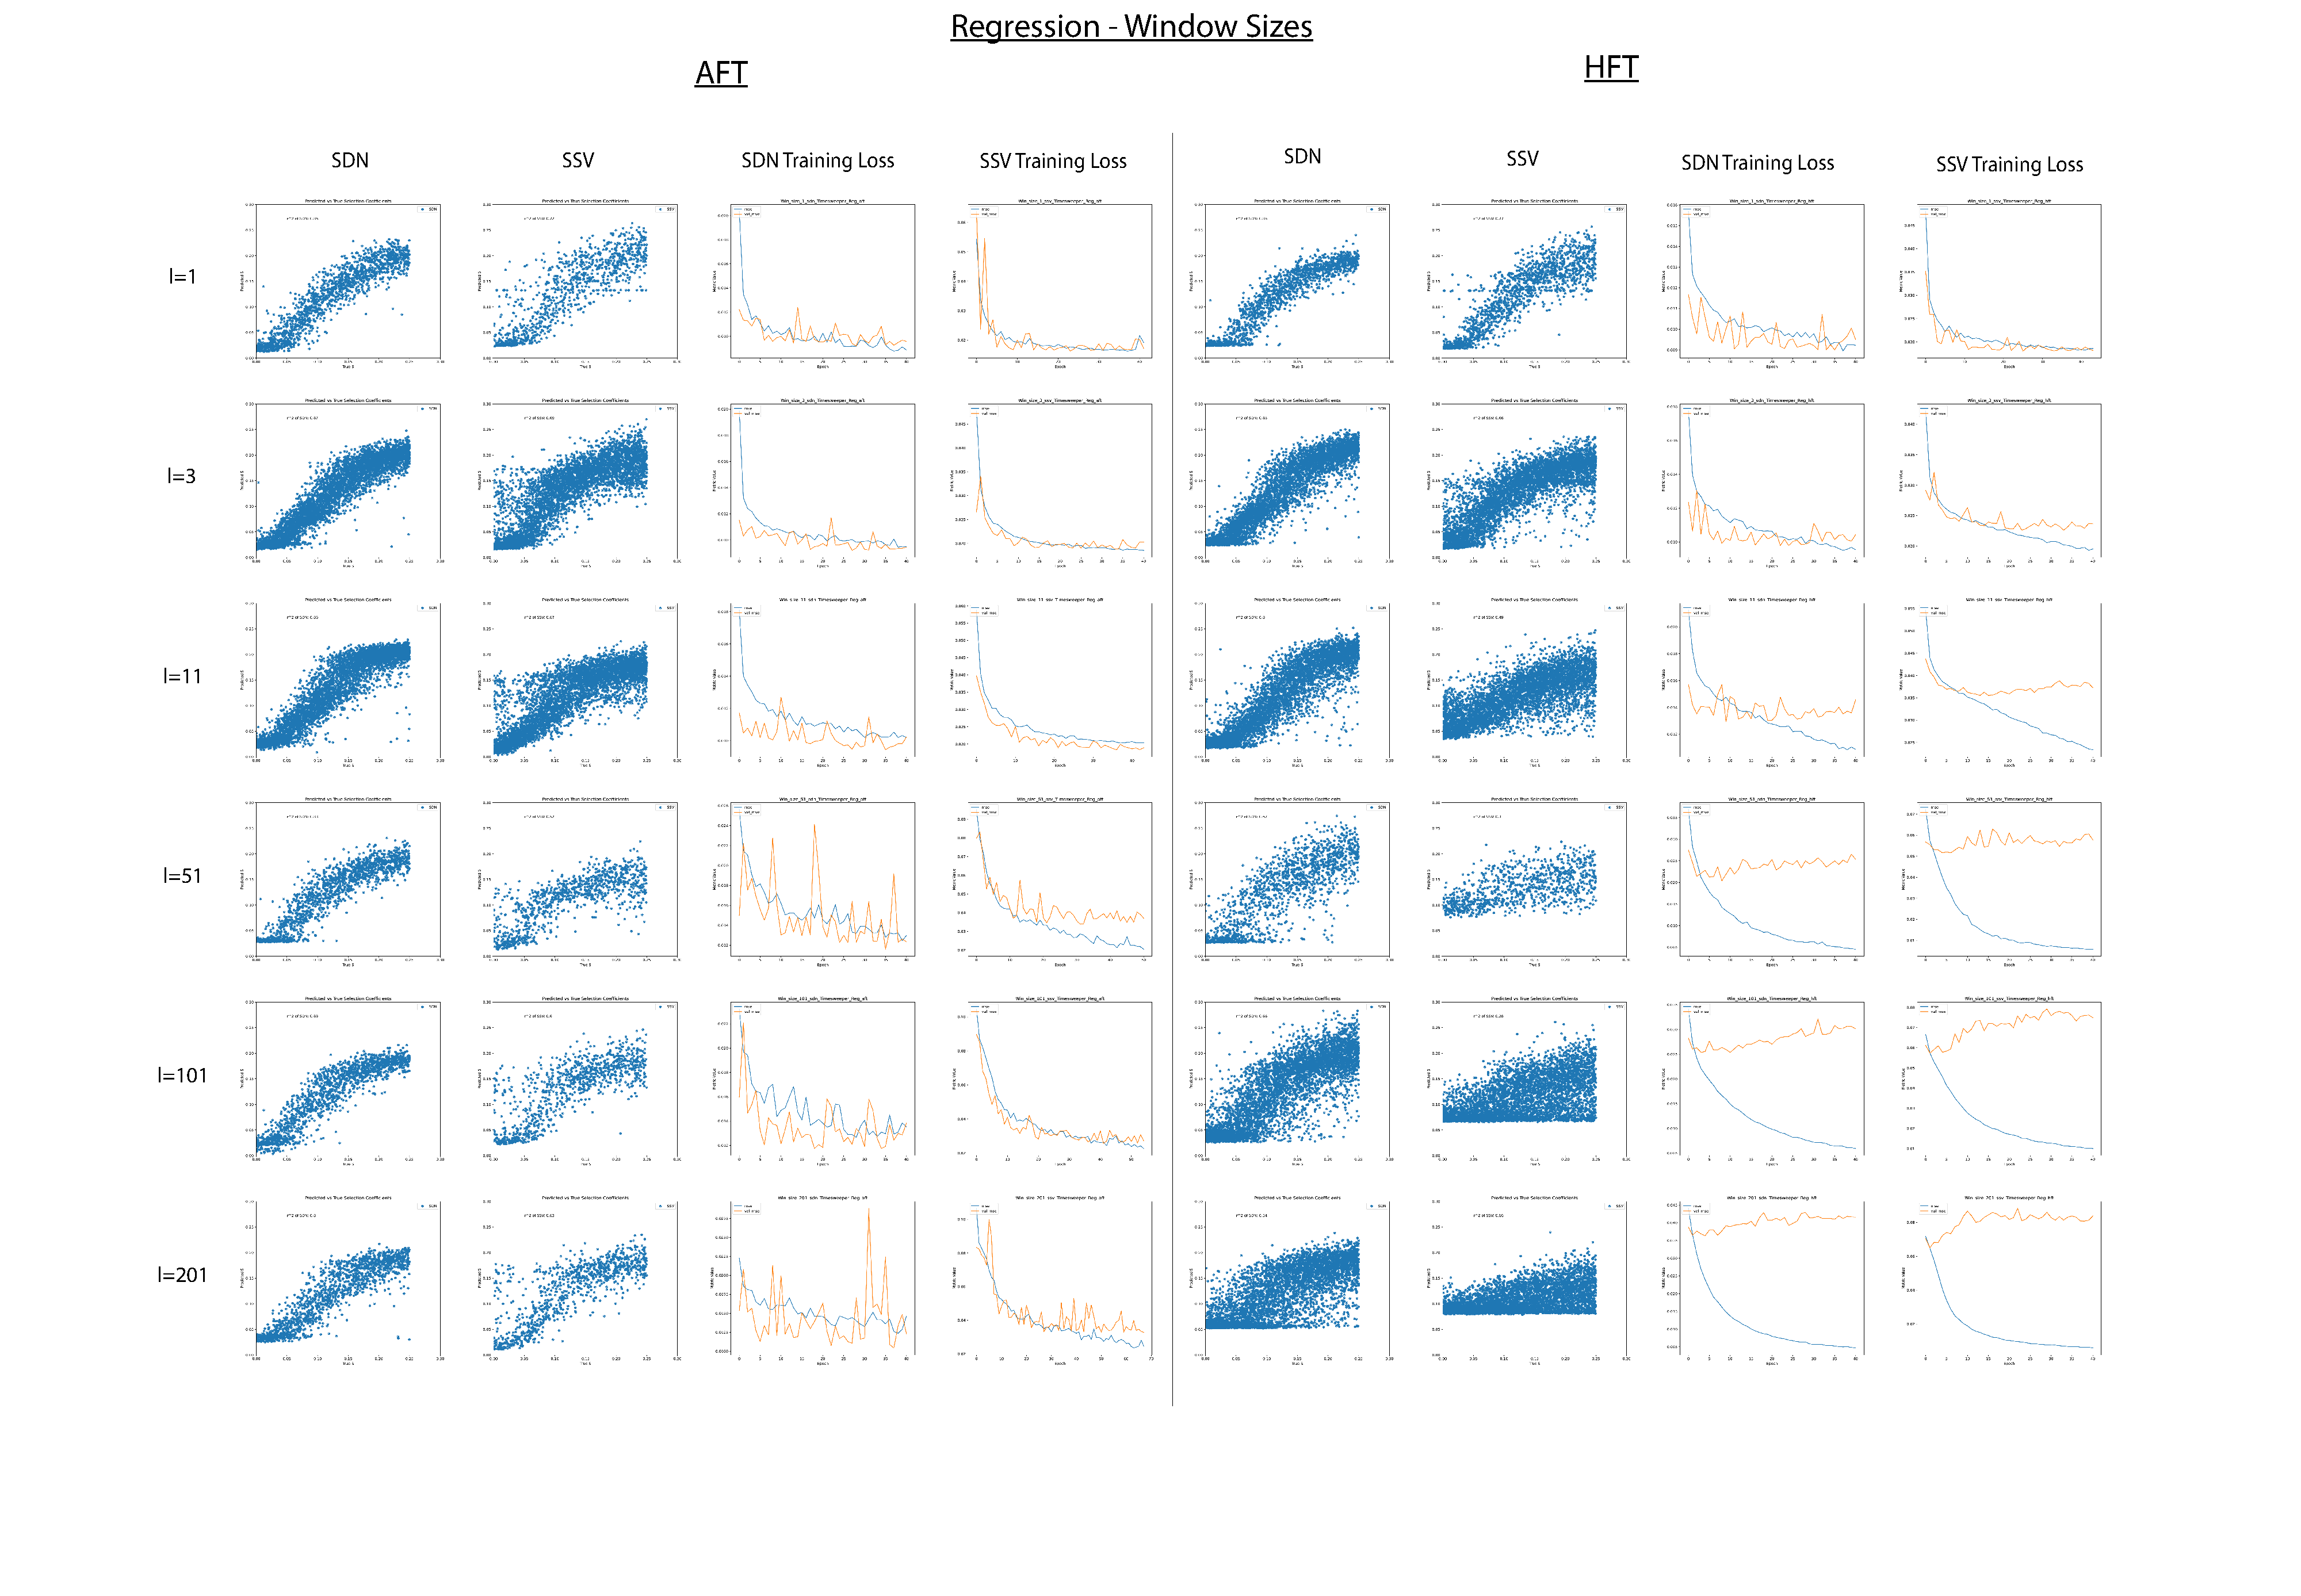
\includegraphics[width=\textwidth]{figures/ap1/S14_Win_Sizes_Reg.pdf}
    \caption[Timesweeper’s classification performance on datasets of varying selection coefficient.]{Timesweeper’s classification performance on datasets of varying selection coefficient. Timesweeper was trained and tested on 10,000 replicates of each scenario (neutrality, SSV, SDN) with a sampling generation drawn from a uniform distribution with bounds [-50, 50) for selection coefficients of 0.005, 0.01, 0.05, 0.1, and 0.5. Precision-recall (PR) curve, ROC curve, Normalized and non-normalized confusion matrices, and training losses for AFT (left half) and HFT (right half) for s values of 0.005, 0.01, 0.05, 0.1, and 0.5.}
    \label{fig:S14_Win_Sizes_Reg}
\end{figure}

\begin{figure}
    \centering
    \includegraphics[width=\textwidth]{figures/ap1/S15_Samp_Size_Class.pdf}
    \caption[ROC Curves for varying selection coefficient classification.]{ROC Curves for varying selection coefficient classification. ROC curves for varying selection coefficients as described in Figure S5 for classifying sweeps versus neutrality (top row) and the SDN scenario versus the SSV scenario (bottom row) for both AFT (left column) and HFT (right column).}
    \label{fig:S15_Samp_Size_Class}
\end{figure}

\begin{figure}
    \centering
    \includegraphics[width=\textwidth]{figures/ap1/S16_Samp_Size_ROC.pdf}
    \caption[PR Curves for varying selection coefficient classification.]{PR Curves for varying selection coefficient classification. PR curves for varying selection coefficients as described in Figure S5 for classifying sweeps versus neutrality (top row) and the SDN scenario versus the SSV scenario (bottom row) for both AFT (left column) and HFT (right column).}
    \label{fig:S16_Samp_Size_ROC}
\end{figure}

\begin{figure}
    \centering
    \includegraphics[width=\textwidth]{figures/ap1/S17_Samp_Size_PR.pdf}
    \caption[Timesweeper’s classification performance using different neural network architectures.]{Timesweeper’s classification performance using different neural network architectures. Timesweeper was trained and tested on the dataset described in Figure S1 using different neural network architectures. PR curves, ROC curves, normalized and non-normalized confusion matrices, and training losses for the classification task (neutrality versus sweep, SDN versus SSV classification) for 1DCNN (top row), 1DCNN with increased parameterization (second row), 2DCNN (third row), and RNN (bottom row) for both AFT (left half) and HFT (right half). }
    \label{fig:S17_Samp_Size_PR}
\end{figure}

\begin{figure}
    \centering
    \includegraphics[width=\textwidth]{figures/ap1/S18_Samp_Size_Reg.pdf}
    \caption[Timesweeper’s selection coefficient-inference performance using different neural network architectures.]{Timesweeper’s selection coefficient-inference performance using different neural network architectures. Timesweeper was benchmarked on a 20-timepoint dataset with selection coefficients drawn from a uniform distribution with bounds [0.00025, 0.25) and a starting sampoint generation drawn from a uniform distribution with bounds [-50, 50) post-selection onset. True s versus estimated s values are plotted for both SDN and SSV scenarios with training losses for each network for 1DCNN (top row), 1DCNN with increased parameterization (second row), 2DCNN (third row), and RNN (bottom row) for both AFT (left half) and HFT (right half).}
    \label{fig:S18_Samp_Size_Reg}
\end{figure}

\begin{figure}
    \centering
    \includegraphics[width=\textwidth]{figures/ap1/S19_TPs_Vary_Class.pdf}
    \caption[Saliency maps of a trained 2DCNN implementation of Timesweeper.]{Saliency maps of a trained 2DCNN implementation of Timesweeper. Saliency maps for the 2DCNN architecture trained on the same benchmark data as described in Figure S8, saliency was calculated using examples from the neutral (left column), SSV (central column), and SDN scenarios (right column) for (A) AFT and (B) HFT data formats.}
    \label{fig:S19_TPs_Vary_Class}
\end{figure}

\begin{figure}
    \centering
    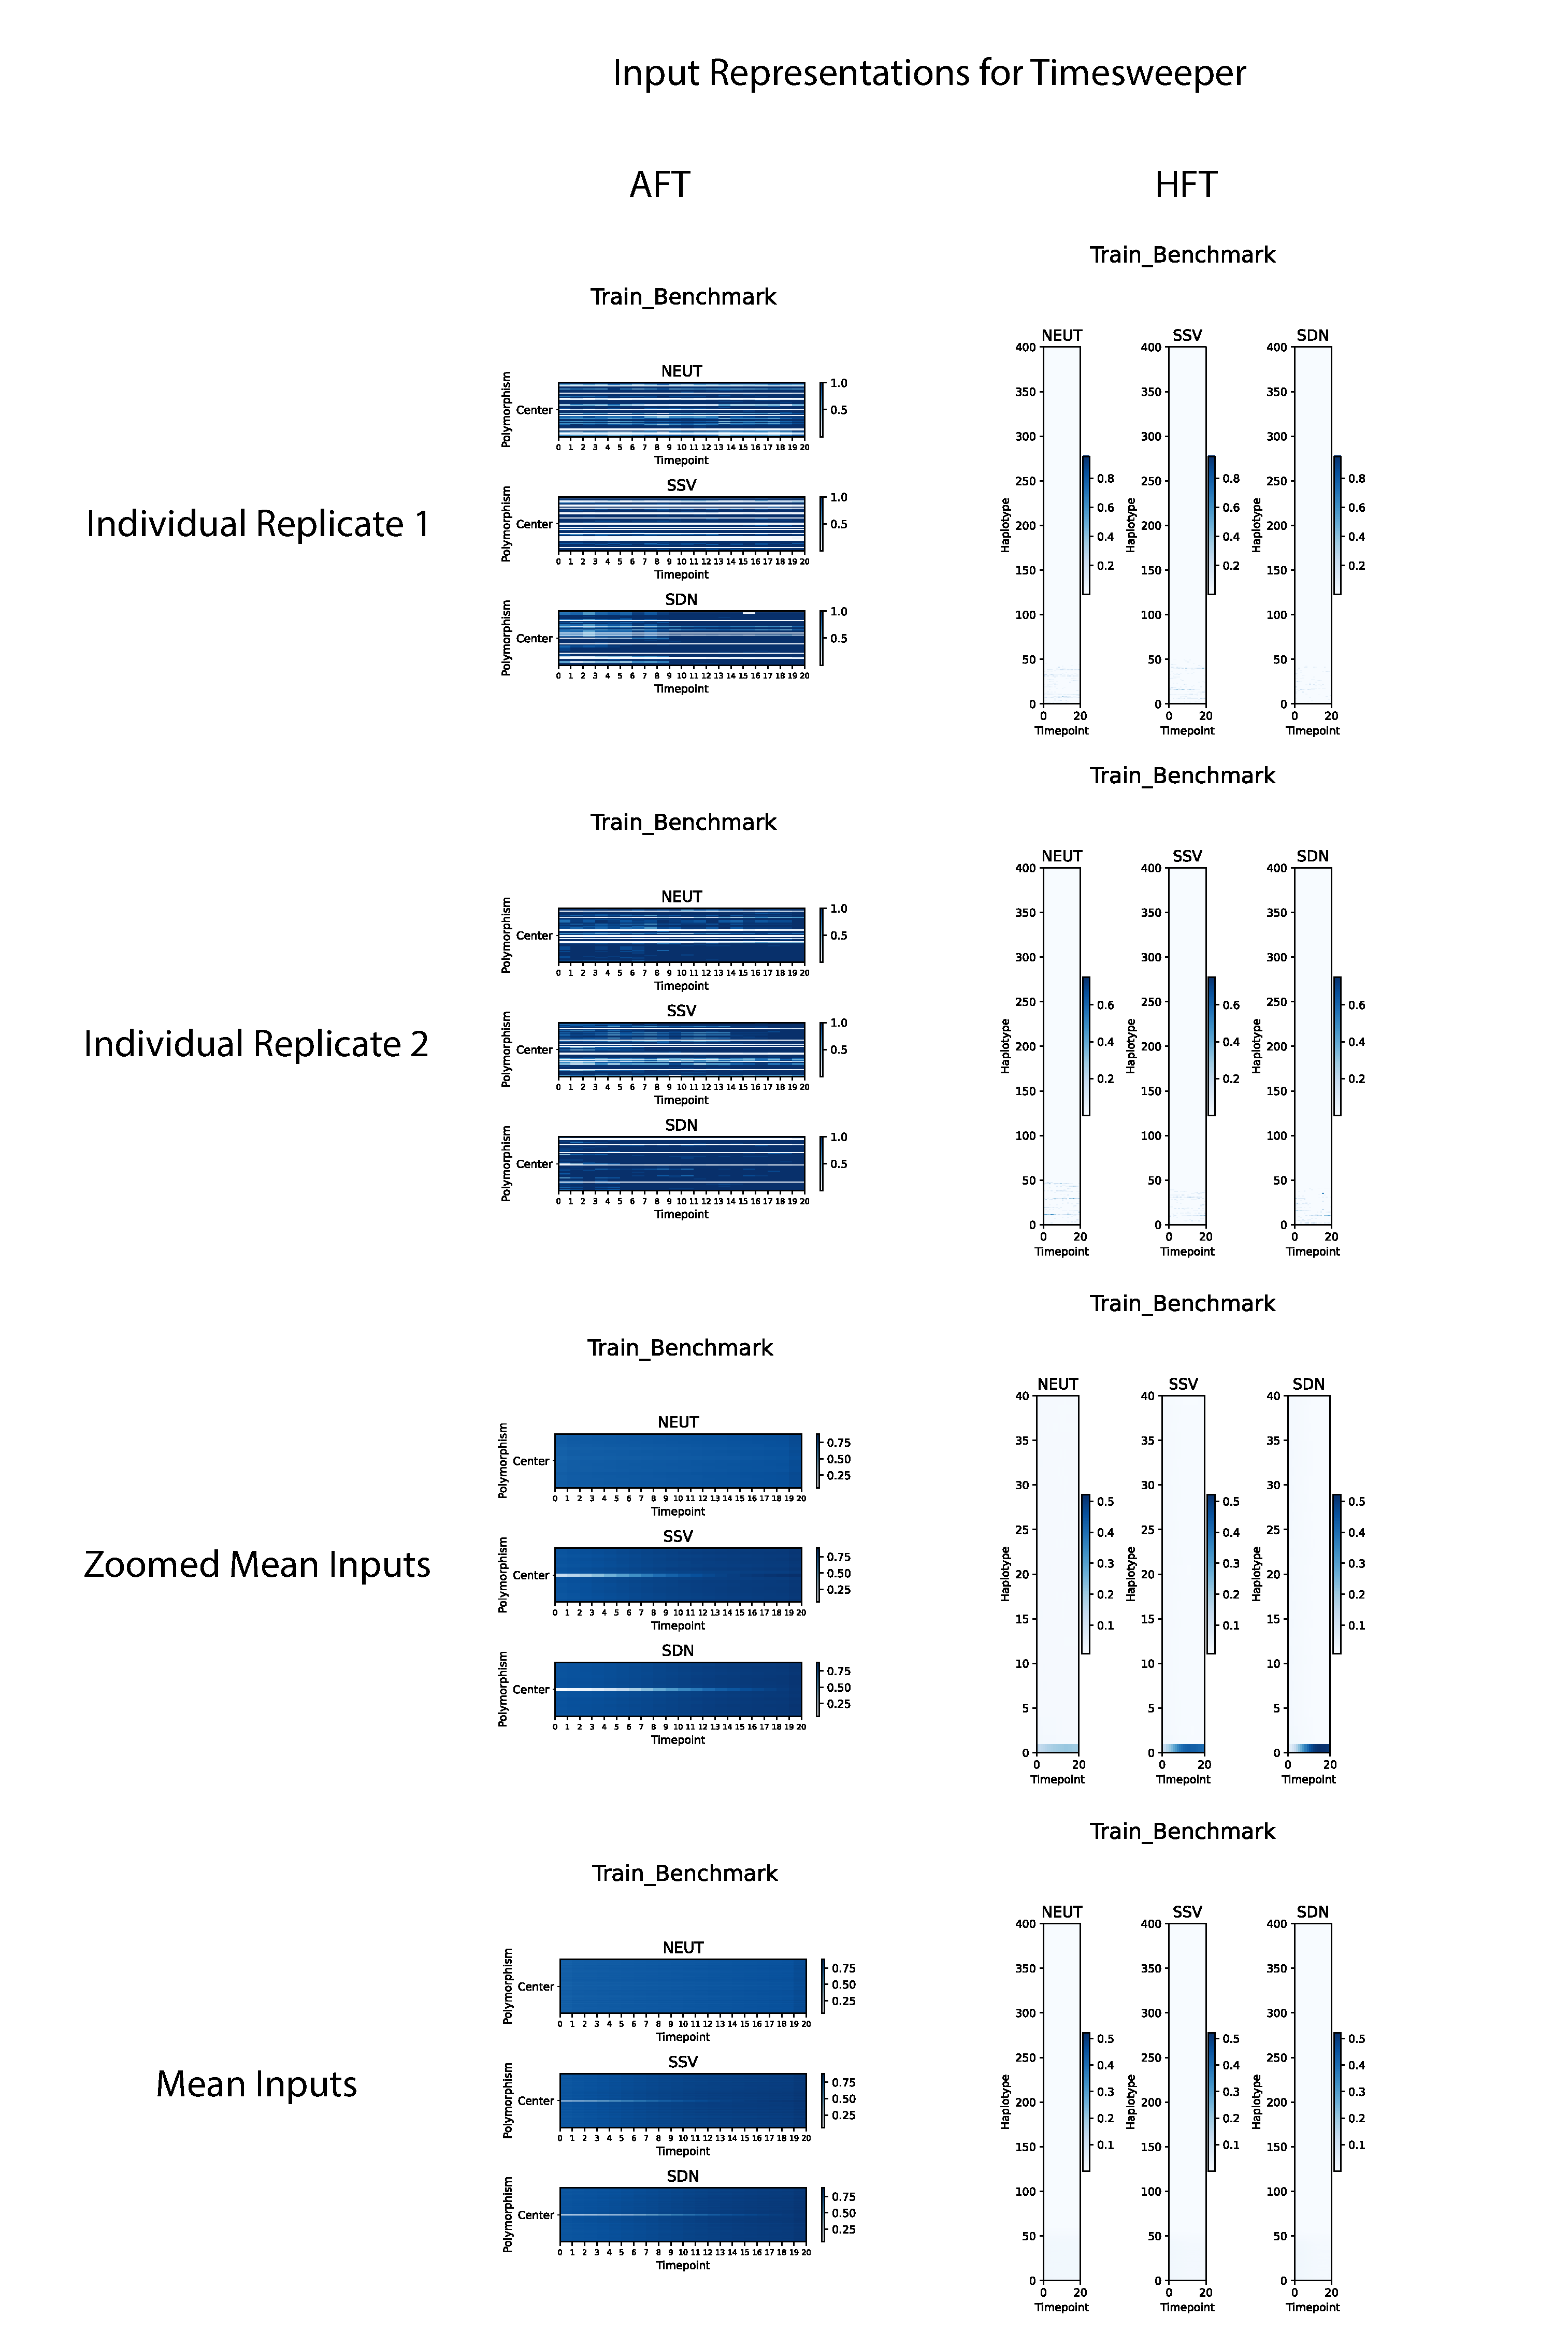
\includegraphics[width=\textwidth]{figures/ap1/S1_All_Inputs.pdf}
    \caption[Timesweeper’s classification performance on a benchmark dataset using different window sizes.]{Timesweeper’s classification performance on a benchmark dataset using different window sizes. Timesweeper was trained and tested on the dataset described in Figure S1 using window sizes of 1, 3, 11, 51, 101, and 201 SNPs. Precision Recall (PR) curve, ROC curve, normalized and non-normalized confusion matrices, and training losses for AFT (left half) and HFT (right half) are displayed for each window size.}
    \label{fig:S1_All_Inputs}
\end{figure}

\begin{figure}
    \centering
    \includegraphics[width=\textwidth]{figures/ap1/S20_TPs_Vary_ROC.pdf}
    \caption[ROC curves for classification performance on datasets with various window sizes.]{ROC curves for classification performance on datasets with various window sizes. Same as Figure S6 but for the data described in Figure S11.}
    \label{fig:S20_TPs_Vary_ROC}
\end{figure}

\begin{figure}
    \centering
    \includegraphics[width=\textwidth]{figures/ap1/S21_TPs_Vary_PR.pdf}
    \caption[PR curves for classification performance on datasets with various window sizes.]{PR curves for classification performance on datasets with various window sizes. Same as Figure S7 but for the data described in Figure S11.}
    \label{fig:S21_TPs_Vary_PR}
\end{figure}

\begin{figure}
    \centering
    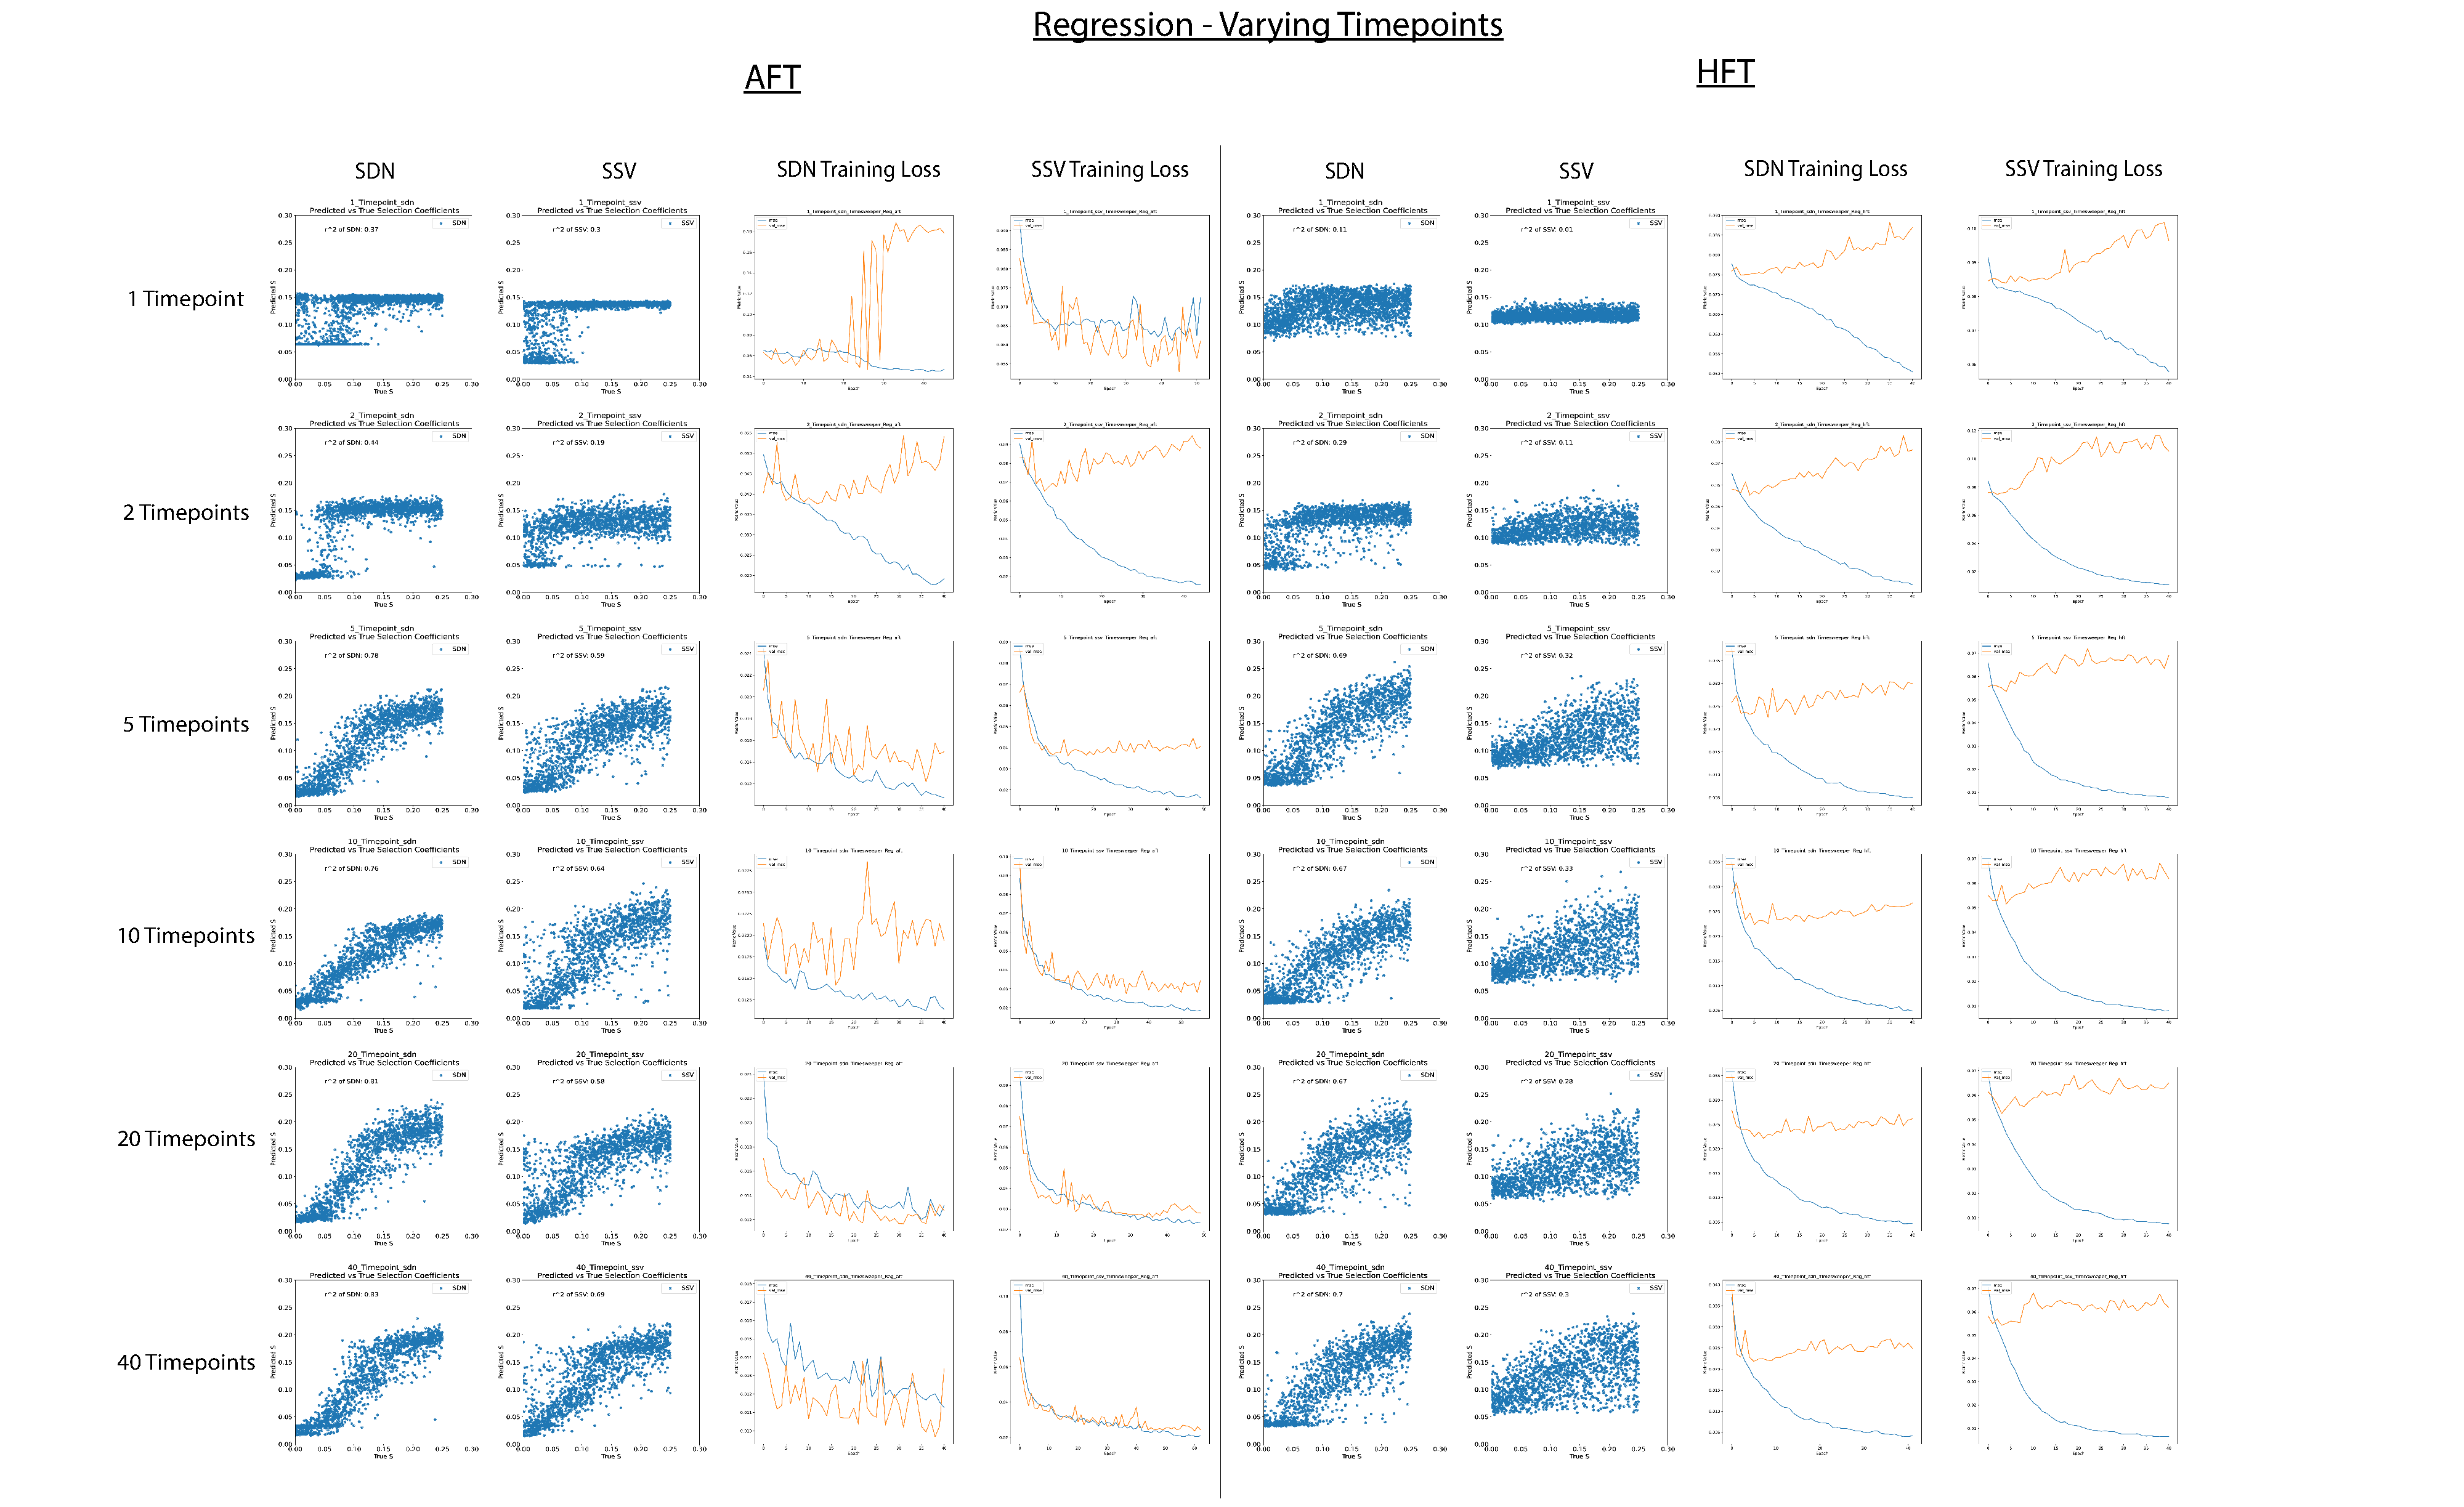
\includegraphics[width=\textwidth]{figures/ap1/S22_TPs_Vary_Reg.pdf}
    \caption[Timesweeper’s regression performance on datasets with various window sizes.]{Timesweeper’s regression performance on datasets with various window sizes. Same as  Figure S9 but for the data described in Figure S11.}
    \label{fig:S22_TPs_Vary_Reg}
\end{figure}

\begin{figure}
    \centering
    \includegraphics[width=\textwidth]{figures/ap1/S23_Sel_Timing_Class.pdf}
    \caption[Timesweeper’s classification performance on datasets with various sample sizes.]{Timesweeper’s classification performance on datasets with various sample sizes. For all simulations 20 timepoints were taken using the same selection coefficient and sampling time parameterization as described in Figure S1. Sample sizes of 1, 2, 5, 10, and 20 individuals were taken at each timepoint. Precision Recall (PR) curve, ROC curve, Normalized and non-normalized confusion matrices, and training losses for AFT (left half) and HFT (right half) are displayed for each sample size.}
    \label{fig:S23_Sel_Timing_Class}
\end{figure}

\begin{figure}
    \centering
    \includegraphics[width=\textwidth]{figures/ap1/S24_Sel_Timing_ROC.pdf}
    \caption[ROC curves for classification performance on datasets with various sample sizes.]{ROC curves for classification performance on datasets with various sample sizes. Same as Figure S6 but for the data described in Figure S15.}
    \label{fig:S24_Sel_Timing_ROC}
\end{figure}

\begin{figure}
    \centering
    \includegraphics[width=\textwidth]{figures/ap1/S25_Sel_Timing_PR.pdf}
    \caption[PR curves for classification performance on datsets with various sample sizes.]{PR curves for classification performance on datsets with various sample sizes. Same as Figure S7 but for the data described in Figure S15.}
    \label{fig:S25_Sel_Timing_PR}
\end{figure}

\begin{figure}
    \centering
    \includegraphics[width=\textwidth]{figures/ap1/S26_Sel_Timing_Reg.pdf}
    \caption[Timesweeper’s regression performance on datasets with various sample sizes.]{Timesweeper’s regression performance on datasets with various sample sizes. Same as  Figure S9 but for the data described in Figure S15.}
    \label{fig:S26_Sel_Timing_Reg}
\end{figure}

\begin{figure}
    \centering
    \includegraphics[width=\textwidth]{figures/ap1/S27_Num_Reps_Class.pdf}
    \caption[Timesweeper’s classification performance on datasets with various numbers of sampled timepoints.]{Timesweeper’s classification performance on datasets with various numbers of sampled timepoints. For all simulations a total of 200 diploid individuals were sampled evenly across the specified number of timepoints (i.e., 200 for the 1-timepoint scenario, 100 per timepoint for the 2-timepoint scenario, etc). Simulation parameterizations for selection coefficient and sampling start time are the same as described in Figure S1. Precision-recall (PR) curve, ROC curve, normalized and non-normalized confusion matrices, and training losses for AFT (left half) and HFT (right half) are displayed for 1, 2, 5, 10, 20, and 40 timepoints.}
    \label{fig:S27_Num_Reps_Class}
\end{figure}

\begin{figure}
    \centering
    \includegraphics[width=\textwidth]{figures/ap1/S28_Num_Reps_ROC.pdf}
    \caption[ROC curves for classification performance on datasets with various numbers of sampled timepoints.]{ROC curves for classification performance on datasets with various numbers of sampled timepoints. Same as Figure S6 but for the data described in Figure S19.}
    \label{fig:S28_Num_Reps_ROC}
\end{figure}

\begin{figure}
    \centering
    \includegraphics[width=\textwidth]{figures/ap1/S29_Num_Reps_PR.pdf}
    \caption[PR curves for classification performance on datasets with various numbers of sampled timepoints.]{PR curves for classification performance on datasets with various numbers of sampled timepoints. Same as Figure S7 but for the data described in Figure S19.}
    \label{fig:S29_Num_Reps_PR}
\end{figure}

\begin{figure}
    \centering
    \includegraphics[width=\textwidth]{figures/ap1/S2_Architectures.png}
    \caption[Timesweeper’s regression performance on datasets with various numbers of sampled timepoints.]{Timesweeper’s regression performance on datasets with various numbers of sampled timepoints. Same as Figure S9 but for the data described in Figure S19.}
    \label{fig:S2_Architectures}
\end{figure}

\begin{figure}
    \centering
    \includegraphics[width=\textwidth]{figures/ap1/S30_Num_Reps_Reg.pdf}
    \caption[Timesweeper’s classification performance on datasets with various sampling start times.]{Timesweeper’s classification performance on datasets with various sampling start times. Simulation parameterizations for selection coefficient are the same as described in Figure S1. Sampling start time was −100,  −50, 0, 25, 100, or 200 generations post-onset of selection. Precision Recall (PR) curve, ROC curve, normalized and non-normalized confusion matrices, and training losses for AFT (left half) and HFT (right half) are displayed.}
    \label{fig:S30_Num_Reps_Reg}
\end{figure}

\begin{figure}
    \centering
    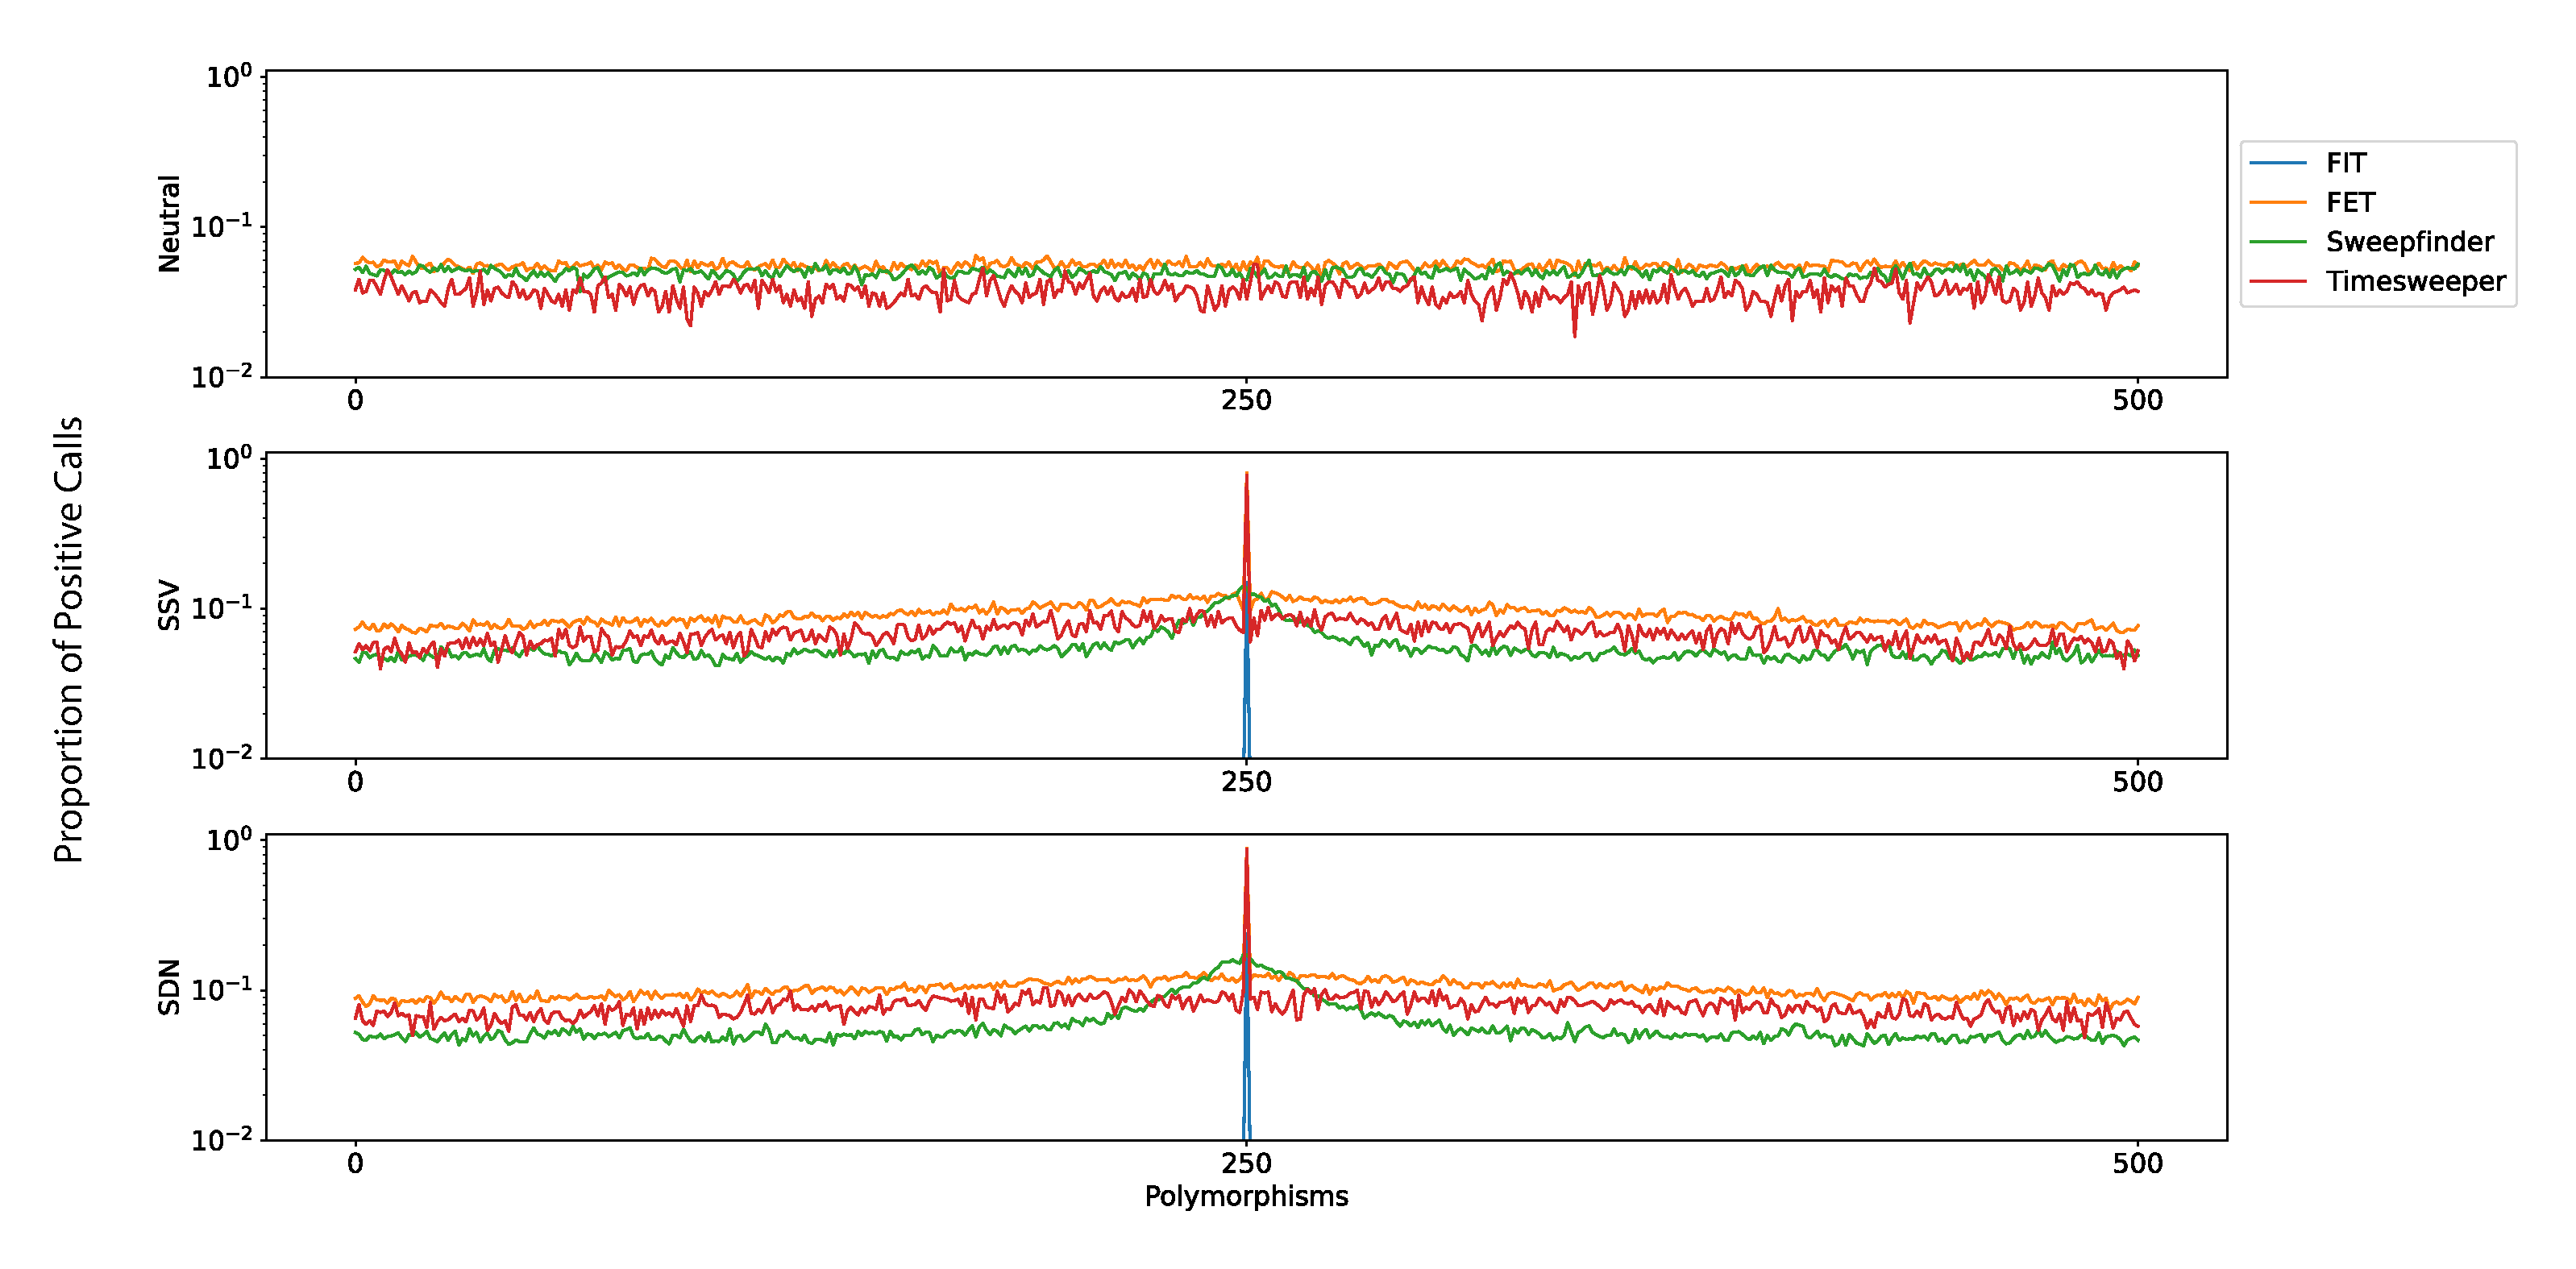
\includegraphics[width=\textwidth]{figures/ap1/S31_Zoomed_Spikes.pdf}
    \caption[ROC curves for classification performance on datasets with various sampling start times.]{ROC curves for classification performance on datasets with various sampling start times. Same as Figure S6 but for the data described in Figure S23.}
    \label{fig:S31_Zoomed_Spikes}
\end{figure}

\begin{figure}
    \centering
    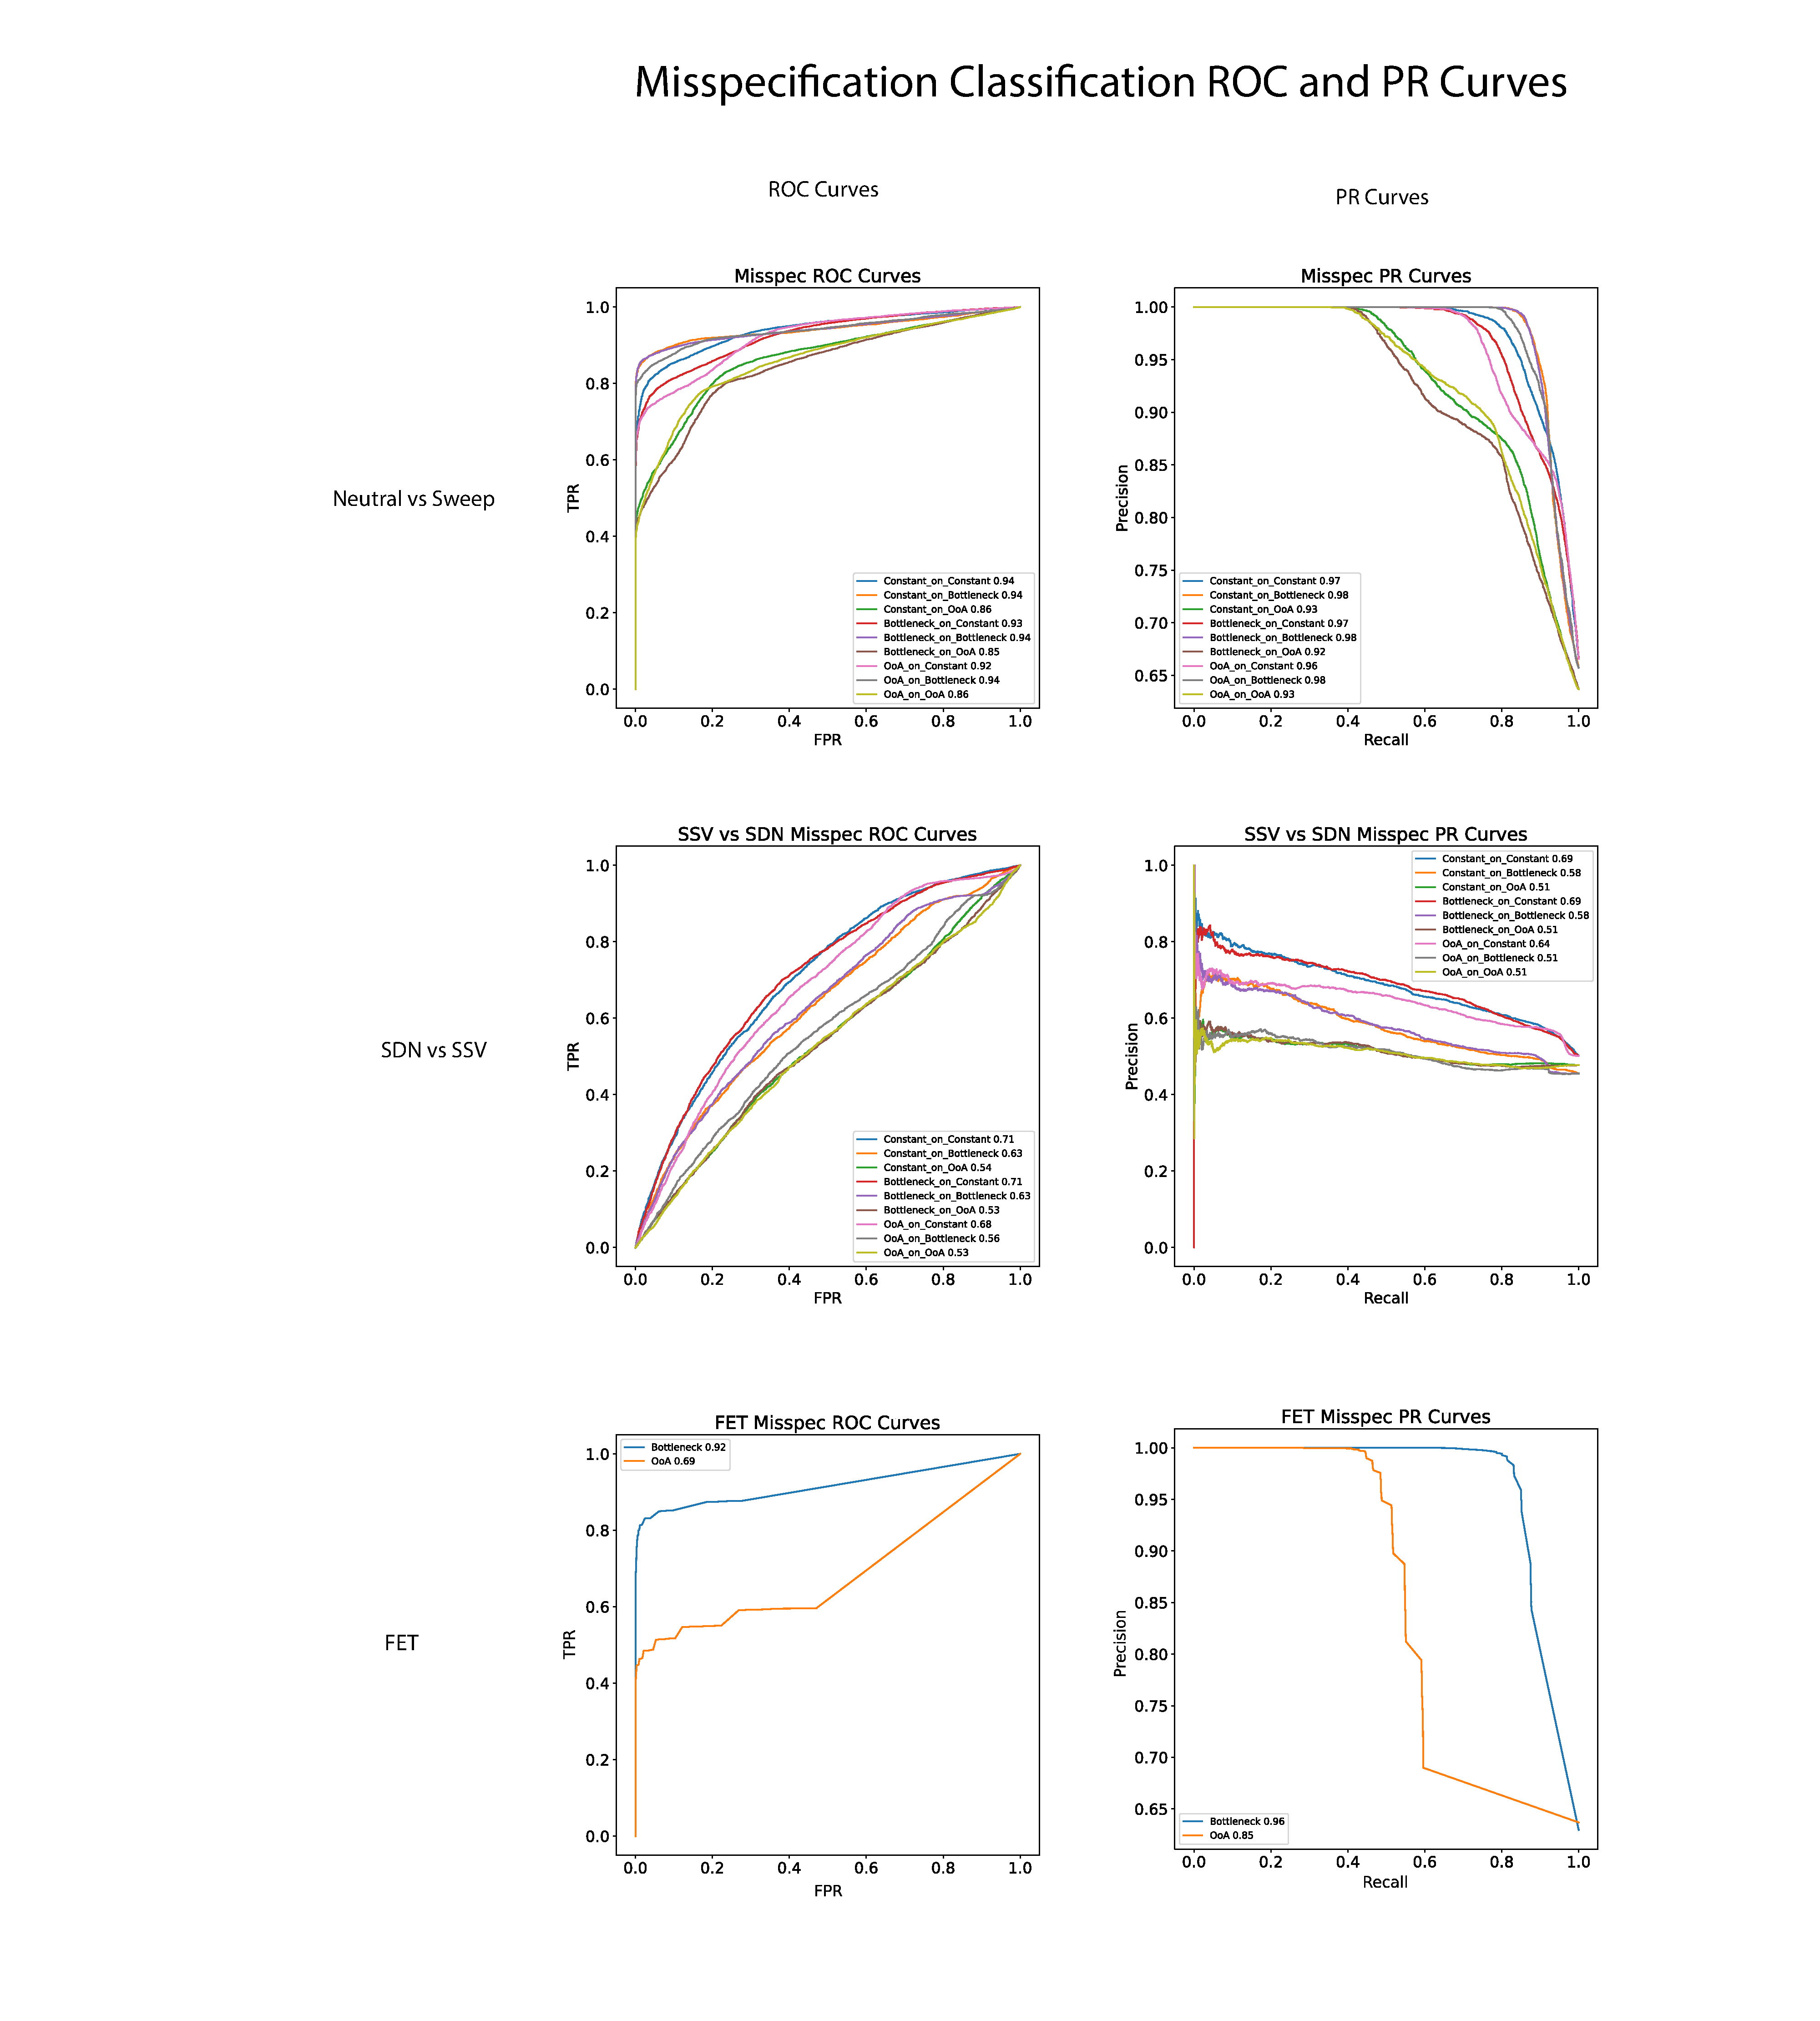
\includegraphics[width=\textwidth]{figures/ap1/S32_Misspec_Classification.pdf}
    \caption[PR curves for classification performance on datasets with various sampling start times.]{PR curves for classification performance on datasets with various sampling start times. Same as Figure S7 but for the data described in Figure S23.}
    \label{fig:S32_Misspec_Classification}
\end{figure}

\begin{figure}
    \centering
    \includegraphics[width=\textwidth]{figures/ap1/S33_Misspec_Regression.pdf}
    \caption[Timesweeper’s regression performance on datasets with various sampling start times.]{Timesweeper’s regression performance on datasets with various sampling start times. Same as Figure S9 but for the data described in Figure S23.}
    \label{fig:S33_Misspec_Regression}
\end{figure}

\begin{figure}
    \centering
    \includegraphics[width=\textwidth]{figures/ap1/S34-D_sim_Inputs.pdf}
    \caption[Timesweeper’s classification performance under various training set sizes.]{Timesweeper’s classification performance under various training set sizes. Simulation parameterizations for selection coefficient and sampling start times are the same as described in Figure S1. Data was subsampled to sizes 30,000, 20,000, 10,000, 5,000, 2,000, and 1,000 for each class (neutral, SSV, SDN). Each dataset was partitioned into training, validation, and test data as described in the Methods. Precision Recall (PR) curve, ROC curve, normalized and non-normalized confusion matrices, and training losses for AFT (left half) and HFT (right half) are displayed.}
    \label{fig:S34-D_sim_Inputs}
\end{figure}

\begin{figure}
    \centering
    \includegraphics[width=\textwidth]{figures/ap1/S35_D_sim_Training_Metrics.pdf}
    \caption[ROC curves for classification performance under various training set sizes.]{ROC curves for classification performance under various training set sizes. Same as Figure S6 but for the data described in Figure S27.}
    \label{fig:S35_D_sim_Training_Metrics}
\end{figure}

\begin{figure}
    \centering
    \includegraphics[width=\textwidth]{figures/ap1/S36_Rep_Hist.pdf}
    \caption[PR curves for  classification performance under various training set sizes.]{PR curves for  classification performance under various training set sizes. Same as Figure S7 but for the data described in Figure S27.}
    \label{fig:S36_Rep_Hist}
\end{figure}

\begin{figure}
    \centering
    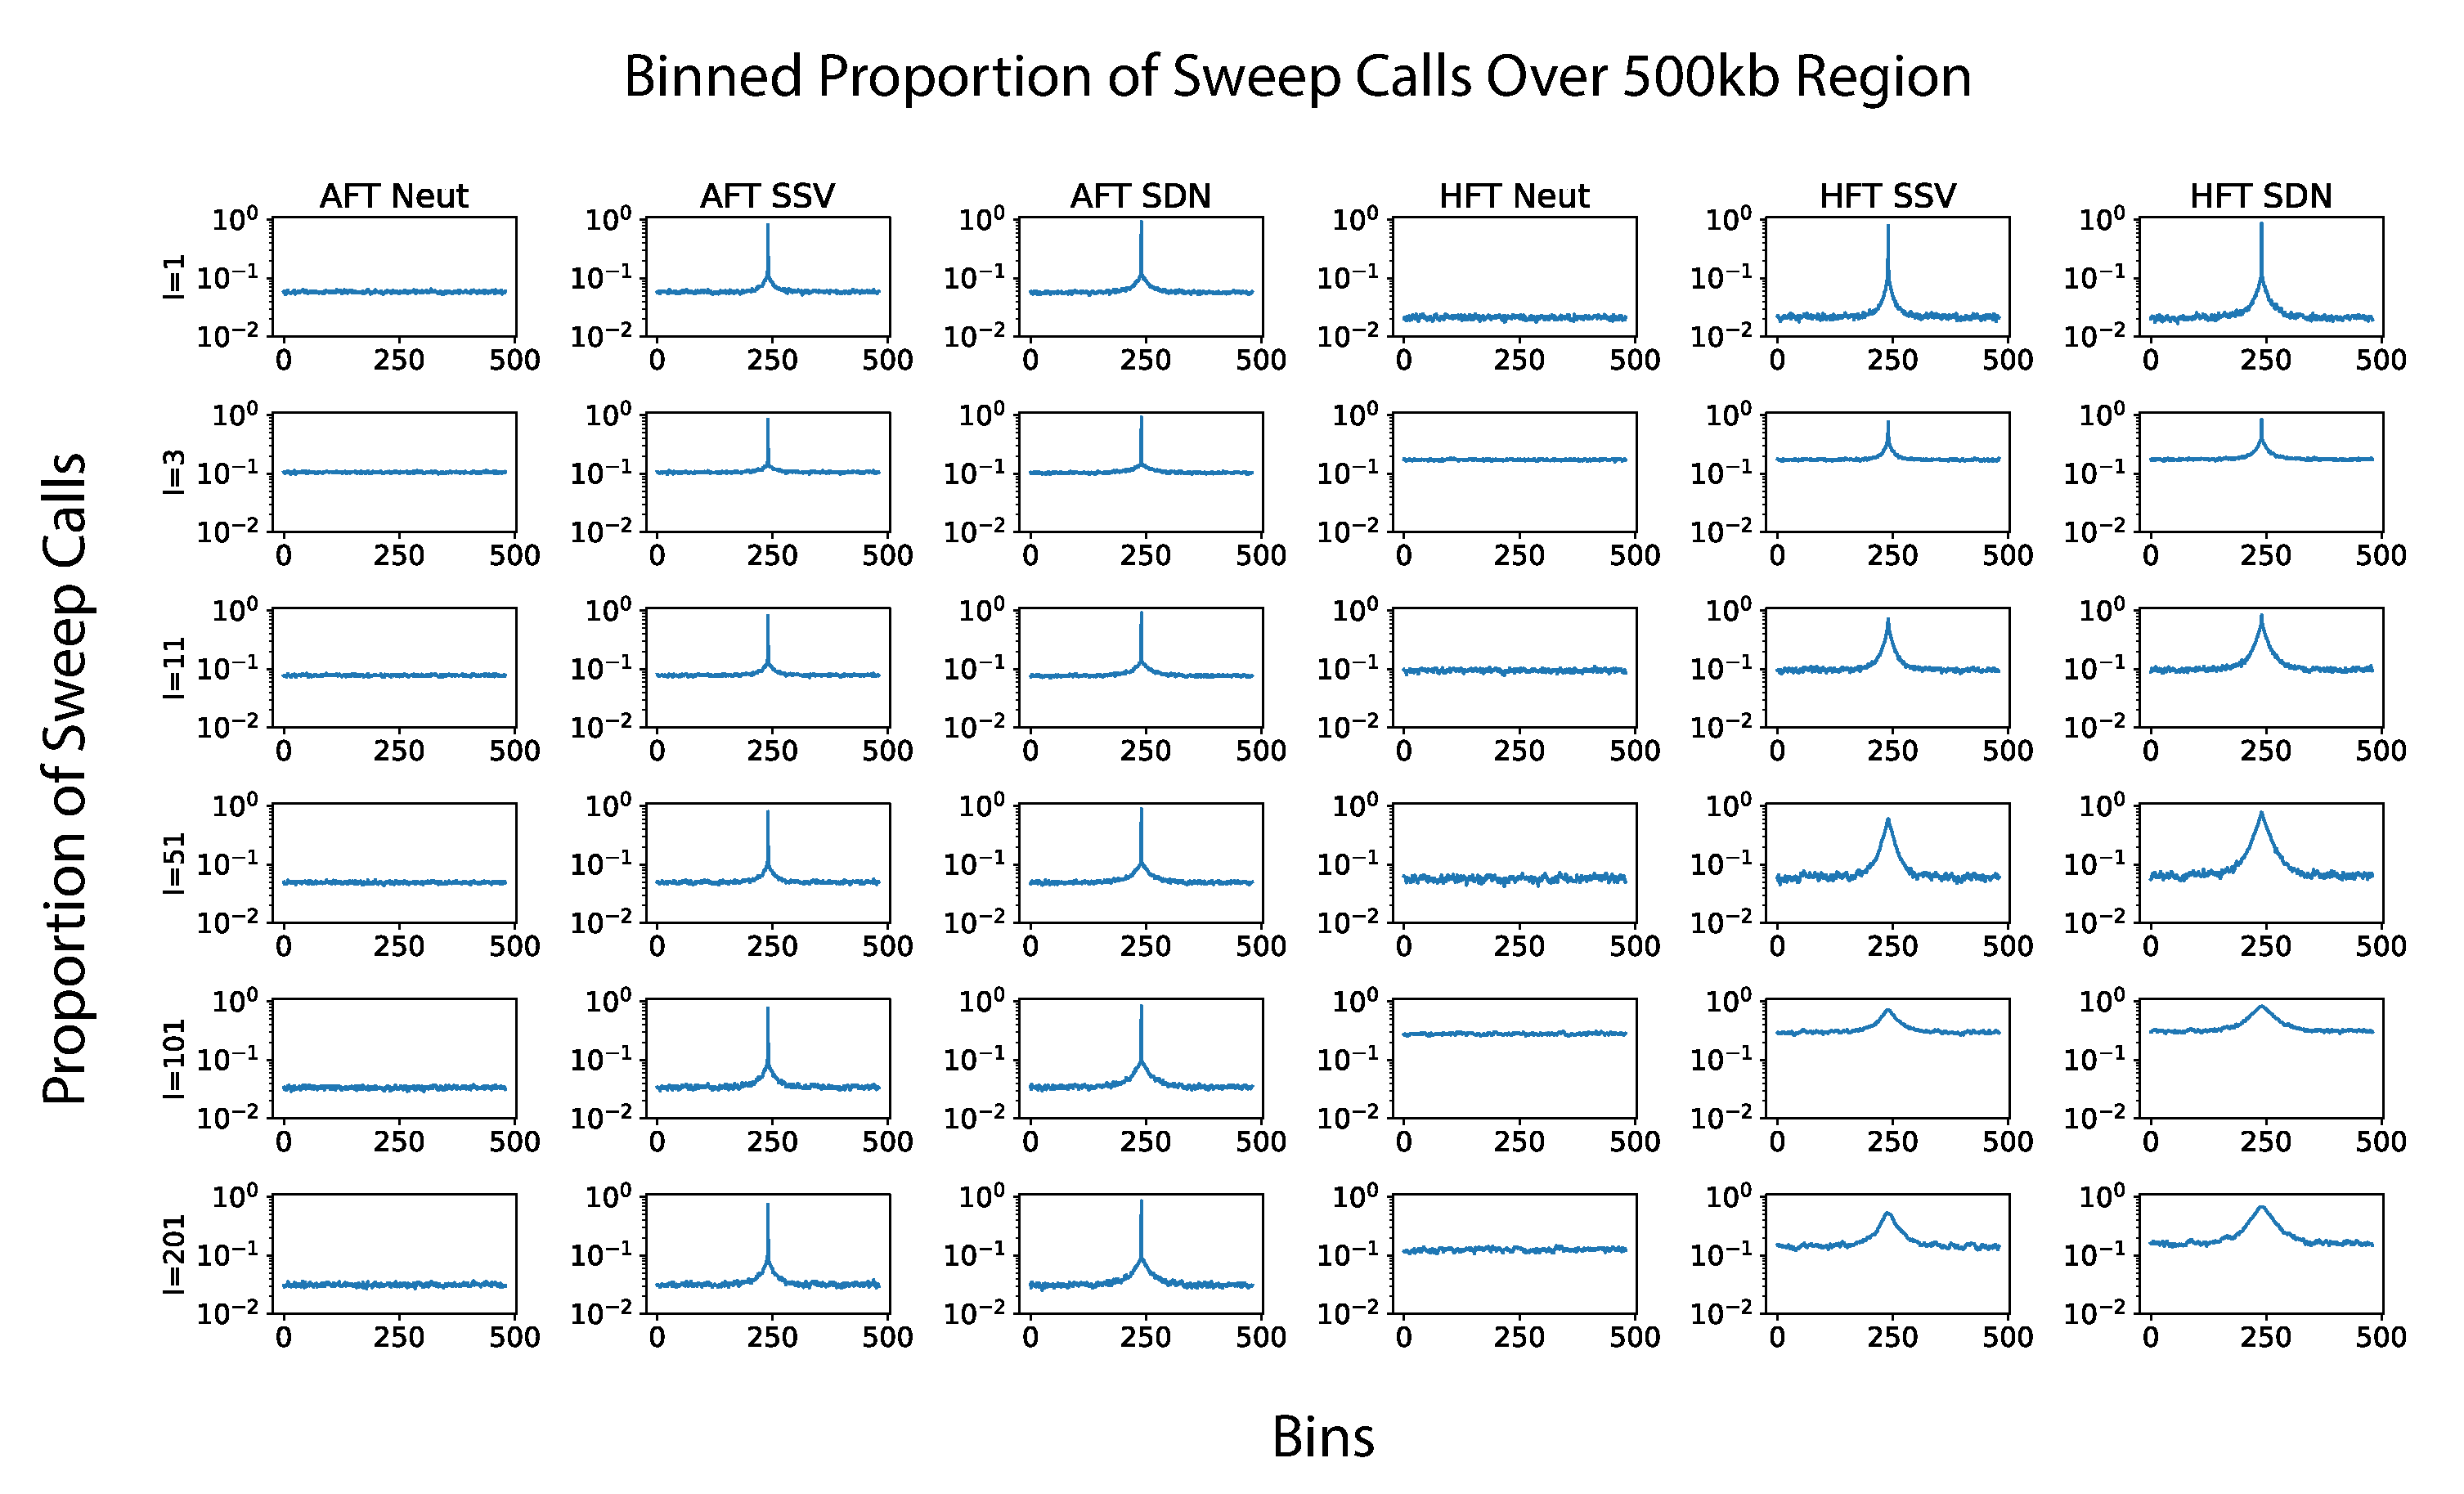
\includegraphics[width=\textwidth]{figures/ap1/S3_Unzoomed_Spikes.pdf}
    \caption[Timesweeper’s regression performance on datasets with varyious training set sizes.]{Timesweeper’s regression performance on datasets with varyious training set sizes. Same as Figure S9 but for the data described in Figure S27.}
    \label{fig:S3_Unzoomed_Spikes}
\end{figure}

\begin{figure}
    \centering
    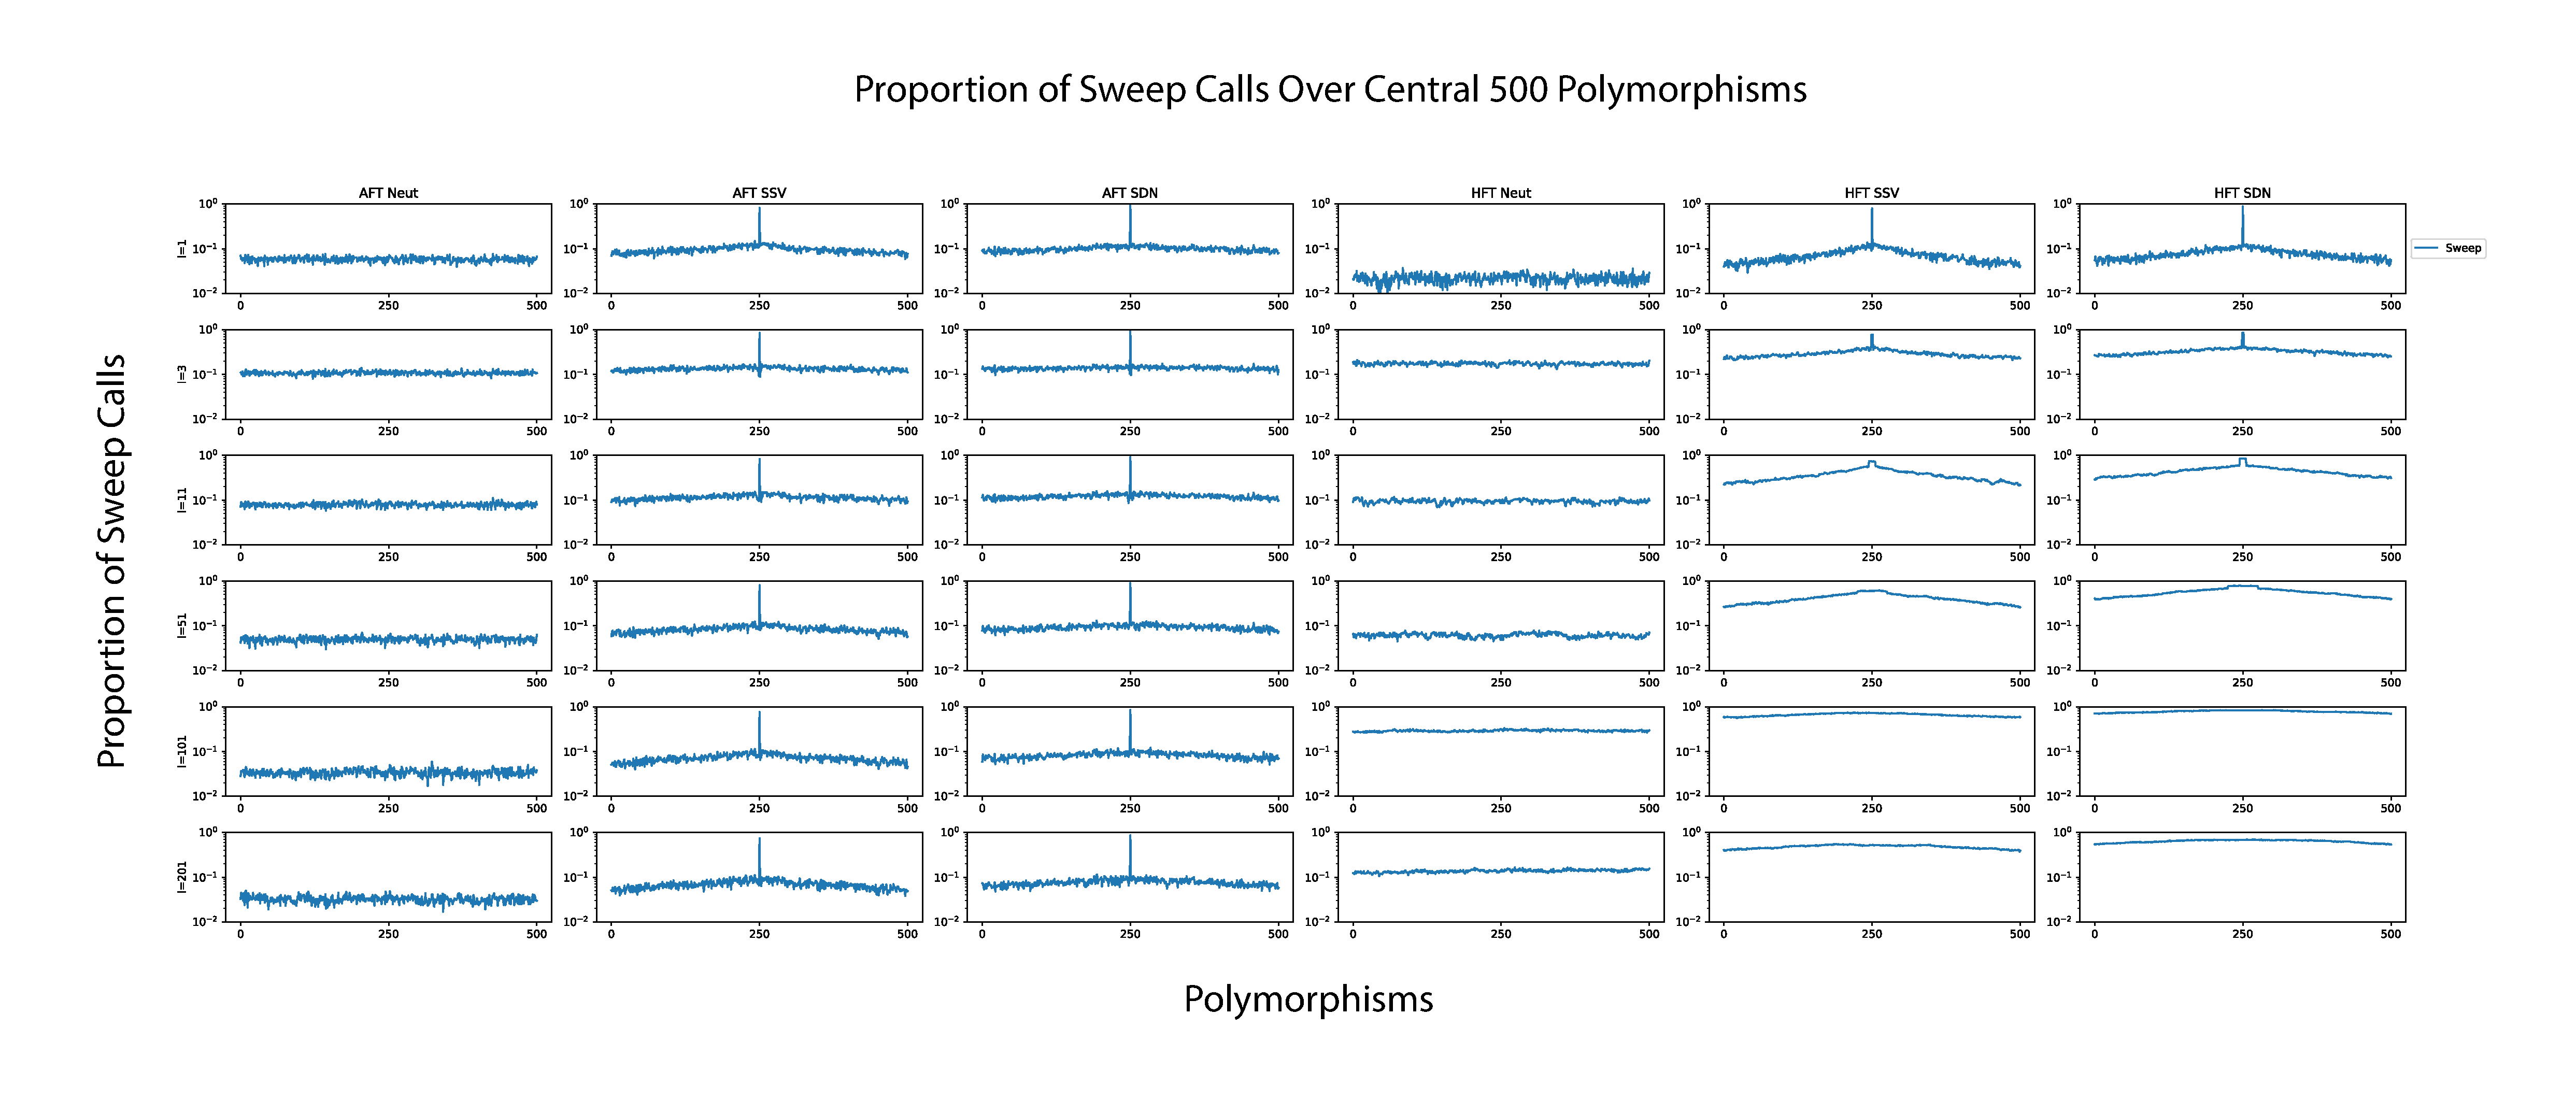
\includegraphics[width=\textwidth]{figures/ap1/S4_Zoomed_Spikes.pdf}
    \caption[Proportion of positive sweep calls for Timesweeper and competing methods, zoomed in towards the center of the window.]{Proportion of positive sweep calls for Timesweeper and competing methods, zoomed in towards the center of the window. The same as Figure S4 but for the data described in Figure 5. }
    \label{fig:S4_Zoomed_Spikes}
\end{figure}

\begin{figure}
    \centering
    \includegraphics[width=\textwidth]{figures/ap1/S5_Sel_Coeff_Class.pdf}
    \caption[Misspecification classification ROC and PR curves.]{Misspecification classification ROC and PR curves. Pairwise ROC (left) and PR (right) curves for neutral versus sweep (top row) and SDN versus SSV (middle row) tasks. The legend specifies the demographic models used for training and testing (in that order) for each curve. FET’s ROC (bottom left) and PR (bottom right) curves are shown for test data simulated under the Bottleneck and OoA models.}
    \label{fig:S5_Sel_Coeff_Class}
\end{figure}

\begin{figure}
    \centering
    \includegraphics[width=\textwidth]{figures/ap1/S6_Sel_Coeff_ROC.pdf}
    \caption[Misspecification regression accuracies.]{Misspecification regression accuracies. Pairwise plots of true versus estimated s for each model trained (rows) and tested on (columns) for both SSV (left) and SDN (right) scenario selection coefficients.}
    \label{fig:S6_Sel_Coeff_ROC}
\end{figure}

\begin{figure}
    \centering
    \includegraphics[width=\textwidth]{figures/ap1/S7_Sel_Coeff_PR.pdf}
    \caption[Example and average Timesweeper inputs from simulated training data for the D.]{Example and average Timesweeper inputs from simulated training data for the \textit{D. simulans} evolve-and-resequence dataset. (A) – (C) show individual example inputs and (D) shows average inputs of the Neutral and SSV classes for the AFT method where data were simulated for the \textit{D. simulans} evolve-and-resequence dataset as described in the Methods.}
    \label{fig:S7_Sel_Coeff_PR}
\end{figure}

\begin{figure}
    \centering
    \includegraphics[width=\textwidth]{figures/ap1/S8_Architectures_Classification.pdf}
    \caption[Timesweeper’s classification performance on simulated test data for the D.]{Timesweeper’s classification performance on simulated test data for the \textit{D. simulans} evolve-and-resequence dataset. (A) – (D) Confusion matrix, ROC curve, training trajectory, and precision-recall (PR) curve showing the performance of the AFT method on simulated \textit{D. simulans} data as described in the Methods.}
    \label{fig:S8_Architectures_Classification}
\end{figure}

\begin{figure}
    \centering
    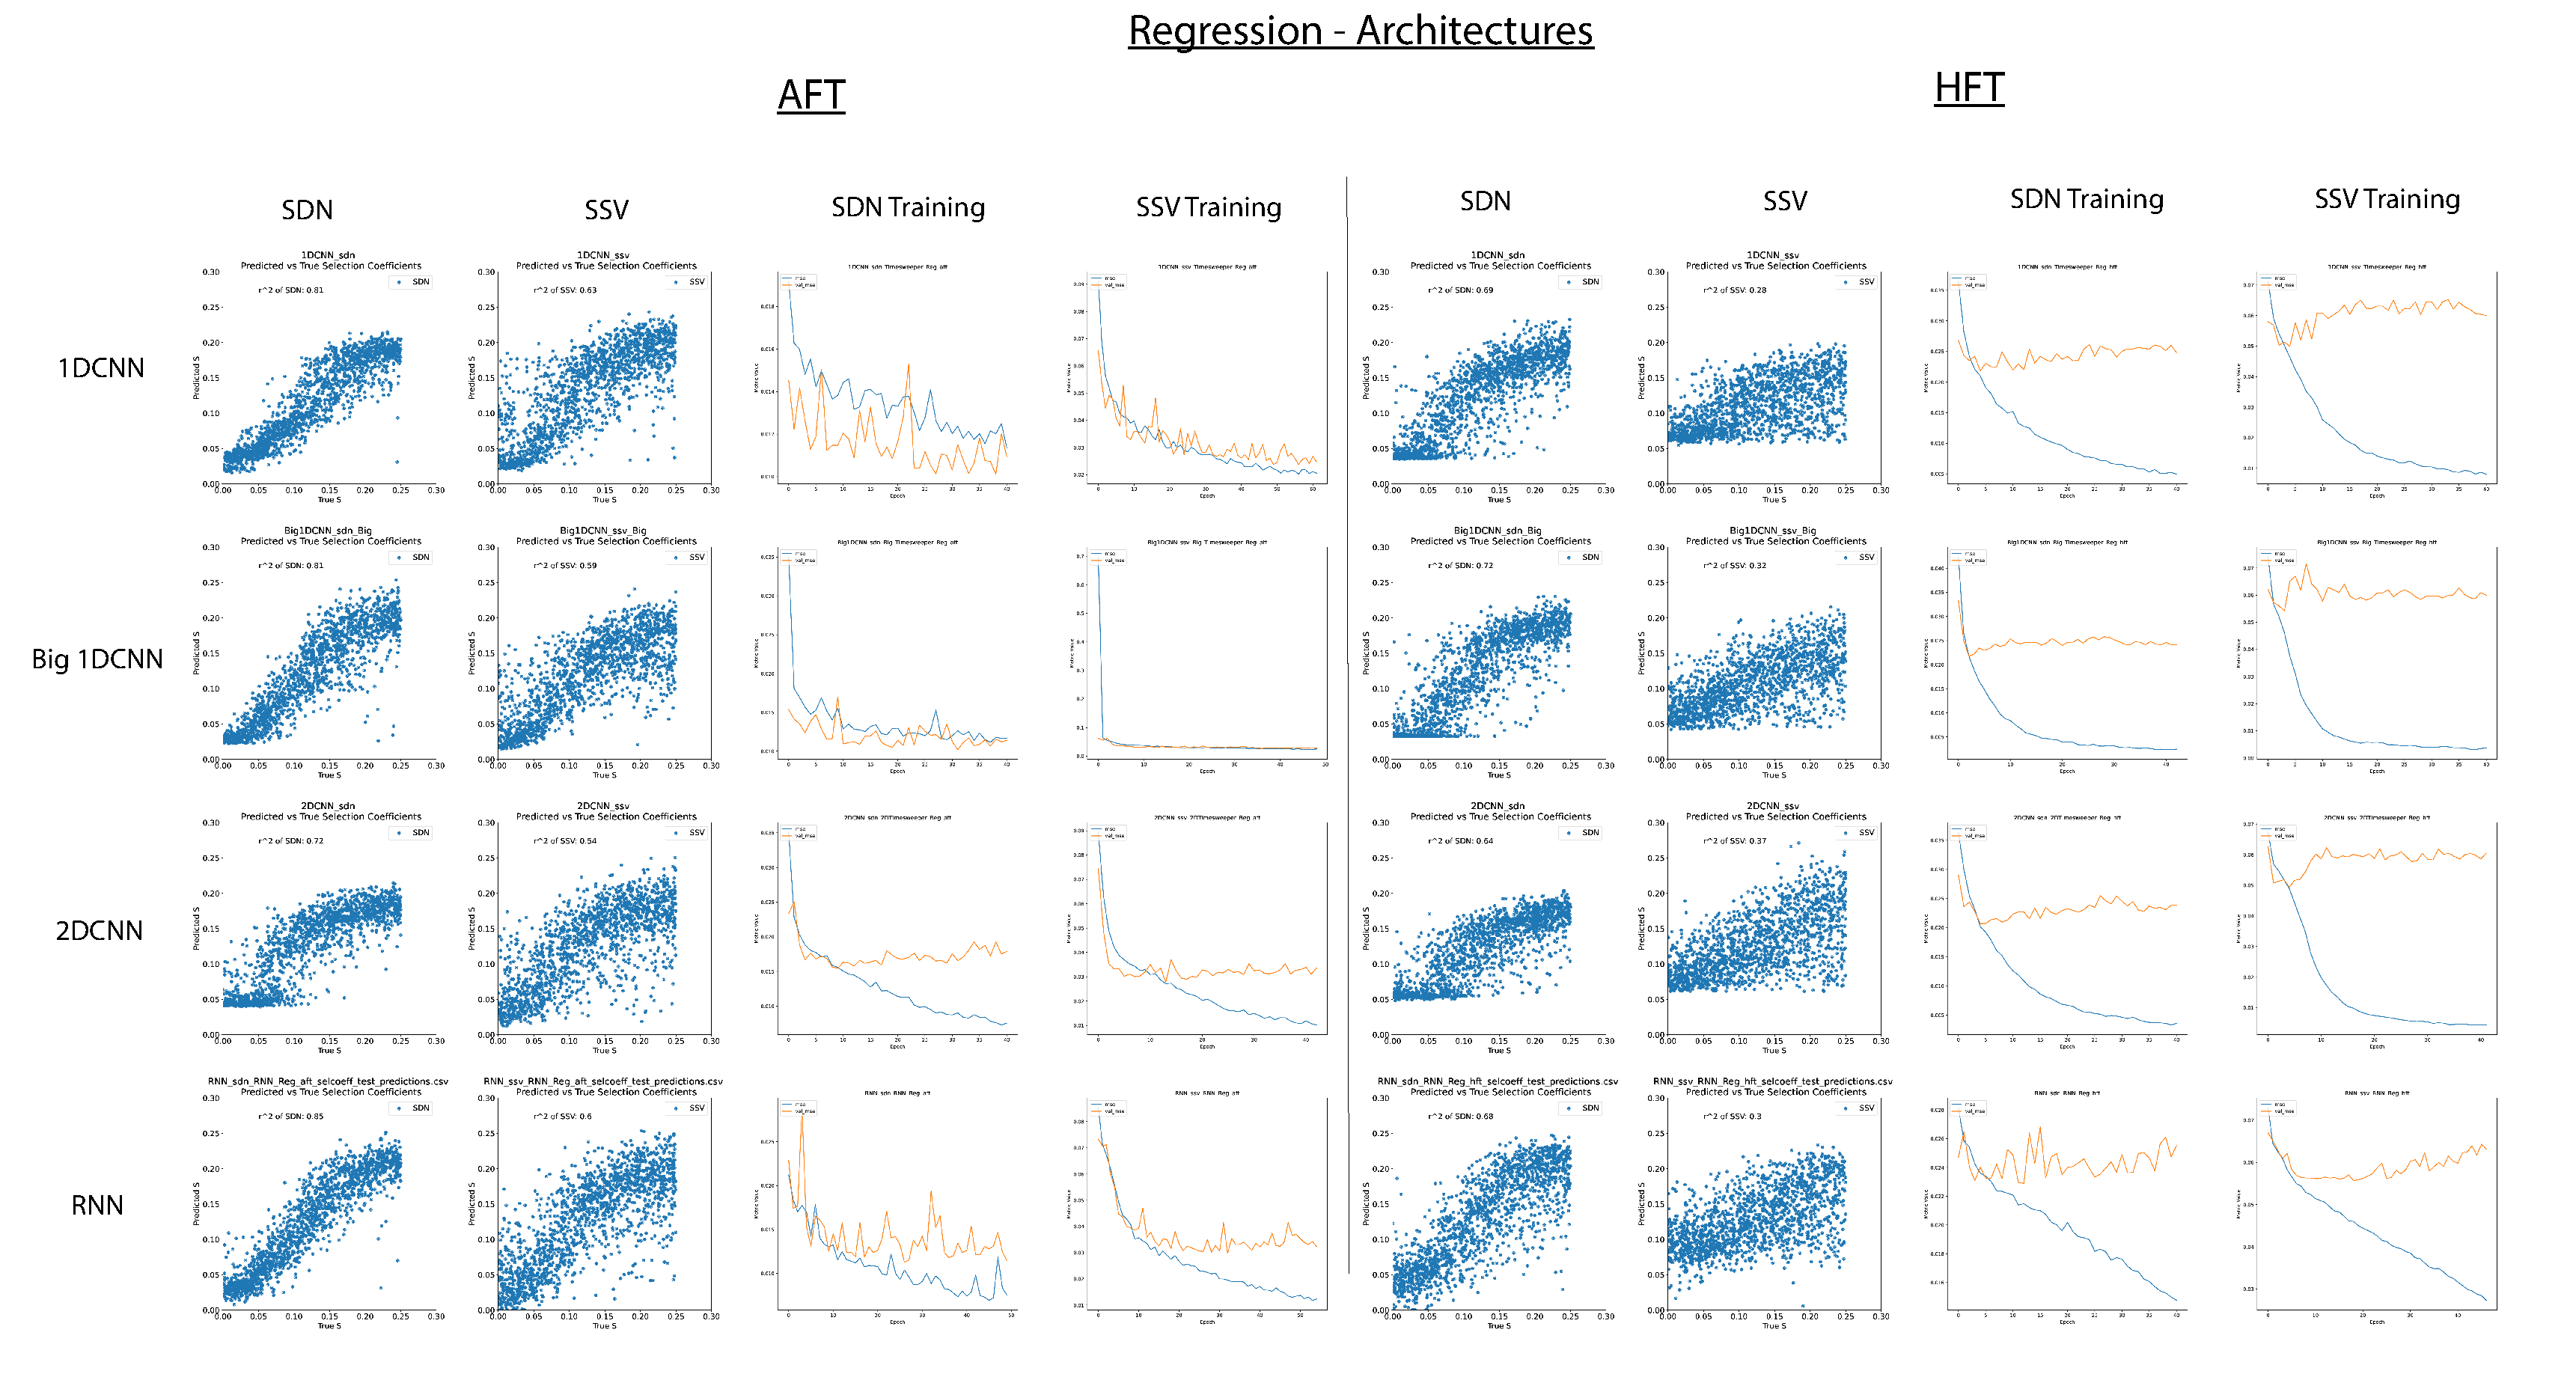
\includegraphics[width=\textwidth]{figures/ap1/S9_Architectures_Regression.pdf}
    \caption[Replication of top hits for Timesweeper and FET in the D.]{Replication of top hits for Timesweeper and FET in the \textit{D. simulans} evolve-and-resequence dataset. A datapoint was counted as replicated sweep if it A) was in the top 100 most confidently-detected sweeps (ranked by Timesweeper sweep probability or by FET 1-pvalue) and B) it occurred in a 100kb window containing at least one outlier SNP (i.e. top 1% of all tested SNPs for a replicate) detected in the other replicate.
}
    \label{fig:S9_Architectures_Regression}
\end{figure}

